\section{Medida de Lebesgue}

\subsection{Medida Exterior de Lebesgue en $\R^n$}

\begin{definición}[n-Réctangulo\label{n-rectángulo}]
Un n-rectángulo en $\R^n$ es un conjunto de la forma:
\begin{equation}
    R = \prod_{i=1}^n [a_i, \ b_i] = [a_1, \ b_1] \times [a_2, \ b_2] \times ... \times [a_n, \ b_n] \text{ donde } a_i \leq b_i \ \forall i
\end{equation}
Definimos el volúmen de $R$ como:
\begin{equation}
    \text{vol}(R) = \prod_{i=1}^n (b_i - a_i)
\end{equation}
Consideramos también los n-rectángulos abiertos denotados por $\mathring{R}$, que se definen de forma análoga. Si nos se especifica si un rectángulo es abierto o cerrado, se asume que es cerrado.
\end{definición}

\begin{observación}
Dado $R$ n-rectángulo cerrado tal que $R = \prod_{i=1}^n [a_i, \ b_i]$, podemos considerar para cada $\delta > 0$ el n-rectángulo abierto $R_\delta = \prod_{i=1}^n (a_i - \delta, \ b_i + \delta)$. Se tiene que $R \subset R_\delta$ y $\text{vol}(R_\delta) = \prod_{i=1}^n (b_i - a_i + 2\delta) = \text{vol}(R) + 2n\delta$. Por tanto:
\begin{equation}
    \text{vol}(R) = \lim_{\delta \to 0} \text{vol}(R_\delta)
\end{equation}
\end{observación}

\begin{definición}[Medida Exterior de Lebesgue\label{Medida de exterior de Lebesgue}]
Sea $A \subset \R^n$. Definimos la medida exterior de $A$ como:
\begin{equation}
    m^*(A) = \inf \left\{ \sum_{i=1}^\infty \text{vol}(R_i) \ | \ A \subset \bigcup_{i=1}^\infty R_i \text{ con } R_i \text{ n-rectángulos cerrados} \right\}
\end{equation}
Donde la ínfimo se toma sobre todas las colecciones numerables de n-rectángulos que recubren $A$. A esta medida exterior la llamamos medida de Lebesgue exterior.
\end{definición}

\begin{observación}
Sea $A \subset \R^n$ entonces:
\vspace{-0.5em}
\begin{enumerate}
    \item $m^*(A) = +\infty \iff \forall (R_j)_{j \in J} \text{ tal que } A \subset \bigcup_{j \in J} R_j \text{ se tiene que } \sum_{j \in J} \text{vol}(R_j) = +\infty$
    \item $m^*(A) = 0 \iff \forall \epsilon > 0 \ \exists (R_j)_{j \in J} \text{ tal que } A \subset \bigcup_{j \ in J} R_j \text{ y } \sum_{j \in J} \text{vol}(R_j) < \epsilon$
    \item $m^*(A) = \alpha \in \R^+ \iff \forall \epsilon > 0 \ \exists (R_j)_{j \in J} \text{ tal que } A \subset \bigcup_{j \in J} R_j \text{ y } \sum_{j \ in J} \text{vol}(R_j) < \alpha + \epsilon$
\end{enumerate}
\end{observación}

\begin{definición}[Conjunto Nulo\label{Conjunto nulo}]
Se dice que $A \subset \R^n$ es un conjunto nulo si $m^*(A) = 0$.
\end{definición}

\ejemplo{
    \begin{enumerate}
        \item Si $R$ es un n-rectángulo degenerado, es decir, $R$ tiene alguno de los lados
              de longitud 0, entonces $R$ es un conjunto nulo ($m^*(R) = 0$).
        \item En $\mathbb{R}^2$, sea el conjunto $A = \{(x,x) : 0 \leq x \leq 1\}$. Dado
              $\epsilon > 0$ tomamos $m \in \mathbb{N}$ tal que $m > \frac{1}{\epsilon}$.
              Consideramos $A \subset \bigcup_{i=1}^m [\frac{i-1}{m}, \frac{i}{m}] \times
                  [\frac{i-1}{m}, \frac{i}{m}]$. Se tiene que $m^*(A) \leq \sum_{i=1}^m
                  \text{vol}([\frac{i-1}{m}, \frac{i}{m}] \times [\frac{i-1}{m}, \frac{i}{m}]) =
                  \frac{1}{m^2} \cdot m = \frac{1}{m} < \epsilon$. Por tanto, $m^*(A) = 0$.
    \end{enumerate}
}

Denotamos por $\mathcal{P}(\R^n)$ al conjunto de todos los subconjuntos de
$\R^n$.
\begin{teorema}
    Sea $m^* \times \mathcal{P}(\R^n) \to [0, +\infty]$ una función que cumple:
    \vspace{-0.5em}
    \begin{enumerate}
        \item $m^*(\emptyset) = 0$
        \item $m^*(A) \leq m^*(B)$ si $A \subset B$
        \item $m^*(\bigcup_{i=1}^\infty A_i) \leq \sum_{i=1}^\infty m^*(A_i)$
    \end{enumerate}
    Entonces $m^*$ es una medida exterior en $\R^n$.
\end{teorema}

\begin{proof}
    % add a space between the proof text and the enumerate
    \leavevmode
    \begin{enumerate}
        \item $\emptyset \subset \bigcup_{i=1}^\infty R_j$ con $R_j$ n-rectángulos degenerados $\implies m^*(\emptyset) \leq \sum_{j=1}^\infty \text{vol}(R_j) = 0 \implies m^*(\emptyset) = 0$.
        \item Sea $A \subset B$ y sea $(R_j)_{j \in J}$ tal que $B \subset \bigcup_{j \in J}
                  R_j$. Entonces $(R_j)_{j \in J}$ es un recubrimiento de $A$ y por tanto $m^*(A)
                  \leq \sum_{j \in J} \text{vol}(R_j) \implies m^*(A) \leq m^*(B)$.
        \item Si $\sum_{j=1}^{\infty}{A_j} = +\infty$ entonces el resultado es inmediato.
              Supongamos que $\sum_{j=1}^{\infty}{A_j} < +\infty$. Sea $\epsilon > 0$. Para
              cada $j \in \mathbb{N}$, $\exists (R_{j,i})_{i = 1}^\infty$ tal que $A_j
                  \subset \bigcup_{i = 1}^\infty R_{j,i}$ y $\sum_{i = 1}^\infty
                  \text{vol}(R_{j,i}) < m^*(A_j) + \frac{\epsilon}{2^j}$. Entonces
              $\bigcup_{j=1}^{\infty} A_j \subset \bigcup_{j=1}^{\infty} \bigcup_{i =
                      1}^\infty R_{j,i}$ y por tanto se tiene que $m^*(\bigcup_{j=1}^{\infty} A_j)
                  \leq \sum_{j=1}^{\infty} \sum_{i = 1}^\infty \text{vol}(R_{j,i}) <
                  \sum_{j=1}^{\infty} (m^*(A_j) + \frac{\epsilon}{2^j})$ = $\sum_{j=1}^{\infty}
                  m^*(A_j) + \epsilon$. Como $\epsilon$ es arbitrario, se tiene que
              $m^*(\bigcup_{j=1}^{\infty} A_j) \leq \sum_{j=1}^{\infty} m^*(A_j)$.
    \end{enumerate}
\end{proof}

\begin{corolario}
    La unión numerable de conjuntos nulos es un conjunto nulo.
\end{corolario}

\begin{proof}
    Sea $(A_j)_{j=1}^\infty \subset R^n$ tal que $m^*(A_j) = 0 \quad \forall j \in \mathbb{N}$ entonces $m^*(\bigcup_{j=1}^\infty A_j) \leq \sum_{j=1}^\infty m^*(A_j) = 0 \implies m^*(\bigcup_{j=1}^\infty A_j) = 0$.
\end{proof}

\begin{lema}
    Sea $A \in \R^n$ entonces $m^*(A) = \inf \left\{ \sum_{i=1}^\infty \text{vol}(Q_i) \ | \ A \subset \bigcup_{i=1}^\infty Q_i \text{ con } Q_i \text{ n-rectángulos abiertos} \right\}$
\end{lema}

\begin{proof}
    Denotamos por $\beta$ el ínfimo de la expresión del enunciado del lema. Sea $(Q_j)_{j \in \N}$ una sucesión de rectángulos abiertos tal que $A \subset \bigcup_{j \in \N} Q_j$. Tenemos entonces que $A \subset \bigcup_{j \in \N} Q_j \subset \bigcup_{j \in \N} \overline{Q}_j$ y puesto que $\sum_{j \in \N} \text{vol}(\overline{Q}_j) = \sum_{j \in \N} \text{vol}(Q_j)$, se tiene que $m^*(A) \leq \sum_{j \in \N} \text{vol}(\overline{Q}_j) \leq \beta$. Por tanto, $m^*(A) \leq \beta$. Veamos ahora la otra desigualdad $\beta \leq m^*(A)$. Si $m^*(A) = +\infty$ entonces $\beta = +\infty$ y no hay nada que demostrar. Supongamos que $m^*(A) < +\infty$. Sea $\epsilon > 0$. Por definición de medida exterior, $\exists (R_j)_{j \in \N}$ sucesión de n-rectángulos cerrados tal que $A \subset \bigcup_{j \in \N} R_j$ y $\sum_{j \in \N} \text{vol}(R_j) < m^*(A) + \epsilon$. Para cada $j \in \N$ consideramos $\epsilon_j = \frac{\epsilon}{2^j}$. Escogiendo $\delta_j > 0$ lo suficientemente pequeño, se tiene que $\text{vol}(R_j)_{\delta_j} < \text{vol}(R_j) + \epsilon_j$ para todo $j \in \N$. Nótese que aquí $\text{vol}(R_j)_{\delta_j}$ denota el volumen del n-rectángulo abierto $R_j$ con lados aumentados en $\delta_j$. Entonces $A \subset \bigcup_{j \in \N} R_j \subset \bigcup_{j \in \N} (R_j)_{\delta_j}$ y $\sum_{j \in \N} \text{vol}(R_j)_{\delta_j} < \sum_{j \in \N} (\text{vol}(R_j) + \epsilon_j) = \sum_{j \in \N} \text{vol}(R_j) + \epsilon < m^*(A) + 2\epsilon$. Por tanto, $\beta \leq m^*(A)$.
\end{proof}

\begin{definición}[Partición de un Conjunto\label{Partición de un Conjunto}]
Una partición del intervalo $[a,b]$ es una colección numerable de puntos $P = \{a = t_0 < t_1 < ... < t_n = b\}$. Dado un n-rectángulo $R \subset \R^n$, una partición $P =  \{P_1, P_2, ..., P_n\}$ de $R$ es una colección particiones $P_i$ de $[a_i, b_i]$ para cada $i = 1, 2, ..., n$ siendo $R = \prod_{i=1}^n [a_i, b_i]$.
\end{definición}

Los subrectángulos de $P$ son los conjuntos de la forma
\begin{equation}
    S_{i_1, i_2, ..., i_n} = \prod_{j=1}^n [t_{i_j}^j, t_{i_j + 1}^j]
\end{equation}
Denotamos $S \in P$ para indicar que $S$ es un subrectángulo de $P$.

\begin{lema}
    Sea $R \subset \R^n$ un n-rectángulo y $P$ una partición de $R$. Entonces:
    \vspace{-0.5em}
    \begin{enumerate}
        \item $R = \bigcup_{S \in P} S$
        \item Si $S, S' \in P$ y $S \neq S'$ entonces $S \cap S' = \emptyset$
        \item $\text{vol}(R) = \sum_{S \in P} \text{vol}(S)$
    \end{enumerate}
\end{lema}

\begin{proposición}
Sea $R \subset \R^n$ un n-rectángulo entonces $m^*(R) = \text{vol}(R)$.
\end{proposición}

\begin{proof}
    \leavevmode\\
    $"\subseteq "$\\
    Sea \( R \subset \bigcup_{j \in \mathbb{N}} R_j \) con \( R_1 = R \) y \( R_j \) degenerados para \( j > 1 \). Entonces:
    \[
        m^*(R) \leq \sum_{j \in \mathbb{N}} \text{vol}(R_j) = \text{vol}(R_1) + \sum_{j=2}^{\infty} \text{vol}(R_j) = \text{vol}(R_1) = \text{vol}(R).
    \]

    $"\supseteq"$\\
    Dado $\epsilon > 0$ existe $(Q_j)_{j \in \mathbb{N}}$ sucesión de n-rectángulos abiertos tal que $R \subset \bigcup_{j \in \mathbb{N}} Q_j$ y $\sum_{j \in \mathbb{N}} \text{vol}(Q_j) < m^*(R) + \epsilon$. Sabemos que R es compacto al ser cerrado y acotado y, por tanto, al ser $\bigcup_{j \in \mathbb{N}} Q_j$ un recubrimiento abierto de R, existe un subrecubrimiento finito $\{Q_1, Q_2, ..., Q_m\}$ de R. Entonces $R \subset \bigcup_{i=1}^m Q_i \subset \bigcup_{i = 1}^m \overline{Q}_i$. Consideramos $R_j = R \cap \overline{Q}_j$ para $j = 1, 2, ..., m$. Tenemos entonces que $R = \bigcup_{j = 1}^{m} \overline{Q}_j$ y además prolongando los lados podemos obtener una partición $P$ de $R$ tal que cada subrectángulo de $P$ está contenido el algún $R_j$ para $1 \leq j \leq m$. Por tanto, $\text{vol}(R) = \sum_{S \in P} \text{vol}(S) \leq \sum_{j = 1}^{m} \text{vol}(R_j) \leq \sum_{j = 1}^{m} \text{vol}(Q_j) < m^*(R) + \epsilon$. Por tanto, $m^*(R) \geq \text{vol}(R)$.
\end{proof}

\subsection{Medida de Lebesgue en $\R^n$}

\textbf{Notación:} Para $A \subset \R^n$ denotamos por $A^c$ al complementario de $A$ en $\R^n$.

\begin{definición}[Conjunto Medible\label{Conjunto Medible}]
Un conjunto $A \subset \R^n$ es medible en el sentido de Lebesgue si para todo $R \subset \R^n$ n-rectángulo se tiene que:
\begin{equation}
    m^*(R) = m^*(R \cap A) + m^*(R \cap A^c)
\end{equation}
\end{definición}

\begin{proposición}
Sea $A \subset \R^n$ entonces son equivalentes:
\vspace{-0.5em}
\begin{enumerate}
    \item $A$ es medible en el sentido de Lebesgue.
    \item $\forall E \subset \R^n$ conjunto se tiene que $m^*(E) = m^*(E \cap A) + m^*(E \cap A^c)$.
    \item $\forall E \subset \R^n$ conjunto se tiene que $m^*(E) \geq m^*(E \cap A) + m^*(E \cap A^c)$.
\end{enumerate}
\end{proposición}

\begin{proof}
    \leavevmode\\
    $"2 \implies 3"$\\
    Trivial\\
    $"3 \implies 2"$\\
    $m^*(E) = m^*(E \cap A) + m^*(E \cap A^c) + m^*(E \cap A \cap A^c) \leq m^*(E \cap A) + m^*(E \cap A^c)$\\
    $"2 \implies 1"$\\
    Inmediato, tomando $E = R$.\\
    $"1 \implies 3"$\\
    Sea $E \subset \R^n$ conjunto, si $m^*(E) = +\infty$ entonces el resultado es inmediato. Supongamos que $m^*(E) < +\infty$. Sea $\epsilon > 0$. Por definición de medida exterior, $\exists (R_j)_{j \in \N}$ sucesión de n-rectángulos cerrados tal que $E \subset \bigcup_{j \in \N} R_j$ y $\sum_{j \in \N} \text{vol}(R_j) < m^*(E) + \epsilon$. Entonces $E \cap A \subset \bigcup_{j \in \N} R_j \cap A$ y $E \cap A^c \subset \bigcup_{j \in \N} R_j \cap A^c$. Por tanto, $m^*(E \cap A) + m^*(E \cap A^c) \leq \sum_{j \in \N} m^*(R_j \cap A) + \sum_{j \in \N} m^*(R_j \cap A^c) = \sum_{j \in \N} \text{vol}(R_j) < m^*(E) + \epsilon$. Por tanto, $m^*(E) \geq m^*(E \cap A) + m^*(E \cap A^c)$.
\end{proof}

\begin{definición}[$\sigma$-Álgebra\label{sigma-Algebra}]
Sea $X$ un conjunto y $\mathcal{A} \subset \mathcal{P}(X)$ una colección de subconjuntos de $X$. Se dice que $\mathcal{A}$ es una $\sigma$-álgebra si:
\vspace{-0.5em}
\begin{enumerate}
    \item $X \in \mathcal{A}$
    \item Si $A \in \mathcal{A} \implies A^c \in \mathcal{A}$
    \item $\forall (A_j)_{j \in \N} \subset \mathcal{A}$ se tiene que $\bigcup_{j \in \N} A_j \in \mathcal{A}$
\end{enumerate}
\end{definición}

\label{Medida}
\begin{definición}[Medida\label{Medida}]
Sea $X$ un conjunto y $\mathcal{A} \subset \mathcal{P}(X)$ una $\sigma$-álgebra, entonces una medida en $X$ es una función $\mu: \mathcal{A} \to [0, +\infty]$ tal que:
\begin{enumerate}
    \item $\mu(\emptyset) = 0$
    \item Si $(A_j)_{j \in \N} \subset \mathcal{A}$ es una colección numerable de
          conjuntos disjuntos dos a dos entonces: $$\mu(\bigcup_{j \in \N} A_j) = \sum_{j
                  \in \N} \mu(A_j)$$
\end{enumerate}
\end{definición}

\begin{teorema}[Medida de Lebesgue en $\R^n$\label{Medida de Lebesgue en Rn}]
    La familia $M$ de todos los conjuntos medibles de $\R^n$ es una $\sigma$-álgebra y $m = m^* \restriction_M$ es una medida numerablemente aditiva que llamaremos medida de Lebesgue en $\R^n$.
\end{teorema}

Demostraremos este teorema con los siguientes lemas:

\begin{lema}
    $\R^n$ es medible en el sentido de Lebesgue.
\end{lema}

\begin{proof}
    Sea $E \subset \R^n$ conjunto. Entonces $m^*(E) = m^*(E \cap \R^n) + m^*(E \cap (\R^n)^c) = m^*(E) + m^*(\emptyset) = m^*(E) + 0 = m^*(E)$.
\end{proof}

\begin{lema}
    Sea $A \subset \R^n$ medible en el sentido de Lebesgue. Entonces $A^c$ es medible en el sentido de Lebesgue.
\end{lema}

\begin{proof}
    Sea $E \subset \R^n$ conjunto. Entonces $m^*(E \cap A^c) + m^*(E \cap (A^c)^c) = m^*(E \cap A^c) + m^*(E \cap A) = m^*(E)$
\end{proof}

Con los dos lemas anteriores obtenemos como colorario que $\emptyset$ es
medible en el sentido de Lebesgue.

\begin{lema}
    Sean $A, B \subset \R^n$ medibles en el sentido de Lebesgue. Entonces $A \cup B$ y $A \cap B$ son medibles en el sentido de Lebesgue.
\end{lema}

\begin{proof}
    Observemos primero que $A \cup B = (A^c \cap B) \cup (A \cap B) \cup (A \cap B^c)$ luego entonces tenemos que $m^*(A \cup B) \leq m^*(A^c \cap B) + m^*(A \cap B) + m^*(A \cap B^c)$. Sea $E \subset \R^n$ conjunto. Entonces $m^*(E) = m^*(E \cap A) + m^*(E \cap A^c) = m^*(E \cap A) + m^*(E \cap A^c \cap B) + m^*(E \cap A^c \cap B^c) = m^*(E \cap A \cap B) + m^*(E \cap A \cap B^c) + m^*(E \cap A^c \cap B) + m^*(E \cap A^c \cap B^c) \geq m^*(E \cap (A \cup B)) + m^*(E \cap A^c \cap B^c) = m^*(E \cap (A \cup B)) + m^*(E \cap (A \cup B)^c).$
\end{proof}

\begin{lema}
    Sea $(A_j)_{j \in \N} \subset \R^n$ una colección numerable de conjuntos medibles en el sentido de Lebesgue. Entonces $\bigcup_{j \in \N} A_j$ es medible en el sentido de Lebesgue y además $m^*(\bigcup_{j \in \N} A_j) = \sum_{j \in \N} m^*(A_j)$.
\end{lema}

\begin{proof}
    Definimos la sucesión creciente de conjuntos $B_k = A_1 \cup \ldots \cup A_k$. Entonces $B_k$ es medible en el sentido de Lebesgue por el lema anterior. Sean $B = \bigcup_{k \in \N} B_k = \bigcup_{j \in \N} A_j$ y $E \in \R^n$ tenemos:
    \[m^*(E \cap B_k) = m^*(E \cap B_k \cap A_k) + m^*(E \cap B_k \cap A_k^c) = m^*(E \cap A_k) + m^*(E \cap B_{k-1}) = m^*(E \cap A_k) + m^*(E \cap B_{k-1})\]
    Reiterando el proceso obtenemos $m^*(E \cap B_k) = \sum_{j=1}^k m^*(E \cap
        A_j)$. Por lo tanto, $m^*(E) = m^*(E \cap B_k) + m^*(E \cap B_k^c) = \left(
        \sum_{j=1}^k m^*(E \cap A_j) \right) + m^*(E \cap B_k^c) \geq \sum_{j=1}^k
        m^*(E \cap A_j) + m^*(E \cap B^c)$. Se sigue entonces $m^*(E) \geq \sum_{j \in
            \N} m^*(E \cap A_j) + m^*(E \cap B^c) \geq m^*(\bigcup_{j \in \N} E \cap A_j) +
        m^*(E \cap B^c) \geq m^*(E \cap B) + m^*(E \cap B^c)$ Luego $B$ es medible.\\
    Tomando $E = B$ en la desigualdad anterior obtenemos $m^*(B) \geq \sum_{j \in
            \N} m^*(B \cap A_j) + m^*(B \cap B^c) = \sum_{j \in \N} m^*(B \cap A_j)$. Por
    otro lado, $m^*(B) \leq \sum_{j \in \N} m^*(B \cap A_j)$ por definición de
    medida exterior. Por tanto, $m^*(B) = \sum_{j \in \N} m^*(A_j) \implies
        m^*(\bigcup_{j \in \N} A_j) = \sum_{j \in \N} m^*(A_j)$.
\end{proof}

\begin{lema}
    La unión numerable de conjuntos medibles en el sentido de Lebesgue es un conjunto medible en el sentido de Lebesgue.
\end{lema}

\begin{proof}
    Sea $(B_j)_{j \in \N}$ una colección numerable de conjuntos medibles en el sentido de Lebesgue. Considermos:
    \[\begin{matrix}
            A_1 = B_1                       \\
            A_2 = B_2 \cap B_1^c            \\
            A_3 = B_3 \cap B_2^c \cap B_1^c \\
            \vdots                          \\
            A_j = B_j \cap B_{j-1}^c \cap \ldots \cap B_1^c
        \end{matrix}\]
    Observemos que $\bigcup_{j \in \N} A_j = \bigcup_{j \in \N} B_j$ y que para
    todo $j \in \N$, $A_j$ es intersección finita de conjuntos medibles, por tanto,
    $A_j$ es medible. Además, $\forall i,j \in \N$ con $i \neq j$, $A_i \cap A_j =
        \emptyset$. Por el lema anterior, $\bigcup_{j \in \N} A_j$ es medible $\implies
        \bigcup_{j \in \N} B_j$ es medible.
\end{proof}

\begin{proposición}
Todo conjunto nulo es medible en el sentido de Lebesgue.
\end{proposición}

\begin{proof}
    Sea $A \subset \R^n$ nulo, entonces $m^*(A) = 0$. $\forall E \in \R^n$ se tiene que $E \cap A \subset A \implies 0 \leq m^*(E \cap A) \leq m^*(A) = 0 \implies m^*(E \cap A) = 0$. Análogamente, $E \cap A^c \subset E \implies 0 \leq m^*(E \cap A^c) \leq m^*(E) \implies m^*(E \cap A^c) = 0$. Por tanto, $m^*(E \cap A) + m^*(E \cap A^c) \leq m^*(E)$. Para la otra desigualdad, $E = (E \cap A) \cup (E \cap A^c) \implies m^*(E) \leq m^*(E \cap A) + m^*(E \cap A^c)$. Y por tanto obtenemos la igualdad $m^*(E) = m^*(E \cap A) + m^*(E \cap A^c)$.
\end{proof}

\begin{definición}[Propiedad en casi todo punto\label{Propiedad en casi todo punto}]
Se dice que una \textit{propiedad} se verifica en casi todo punto cuando el conjunto de puntos en los que no se verifica la propiedad es un conjunto nulo.
\end{definición}

\begin{proposición}
Todo n-rectángulo cerrado $R \in \R^n$ es medible en el sentido de Lebesgue.
\end{proposición}

\begin{proof}
    Dado $R \subset \R^n$ n-rectángulo cerrado, tenemos que ver que $\forall Q \in \R^n$ n-rectángulo cerrado se tiene que $\text{vol}(Q) \geq m^*(Q \cap R) + m^*(Q \cap R^c)$. Consideramos el n-rectángulo $Q_0 = Q \cap R$. Nótese que $Q \cap R^c$ es unión finita de n-rectángulos $\{Q_1,\ldots, Q_m\}$. Entonces $Q = Q_0 \cup Q_1 \cup \ldots \cup Q_m$ forman una partición de $Q$. Luego $\text{vol}(Q) = \sum_{i=0}^m \text{vol}(Q_i) = m^*(Q \cap R) + \sum_{i=1}^m m^*(Q_i) \geq m^*(Q \cap R) + m^*(Q \cap R^c)$.
\end{proof}

\begin{observación}
En $\R^n$ los rectángulos abiertos son medibles en el sentido de Lebesgue.
\end{observación}

\begin{definición}[n-Cubo\label{n-Cubo}]
Un n-cubo cerrado (respectivamente abierto) en $\R^n$ es un conjunto de la forma:
\begin{equation}
    R = [a_1, b_1] \times \ldots \times [a_n, b_n] \text{ tal que } \forall i,j \in \{1,2,...,n\} \text{ se tiene que } b_i - a_i = b_j - a_j
\end{equation}
Análogamente se pueden definir los cubos n-dimensionales semi-abiertos.
\end{definición}

\observacion{
    Denotaremos la norma del supremo en $\rn$ como:
    \begin{equation}
        ||x||_{\infty} = \sup_{i=1}^n \{|x_i|\} \text{ para } x = (x_1, x_2, ..., x_n) \in \rn
    \end{equation}
    Llamaremos bola abierta de centro $x \in \rn$ y radio $r > 0$ al conjunto:
    \begin{equation}
        B_{\infty}(x, r) = \{y \in \rn : ||y - x||_{\infty} < r\} \equiv (x_1 - r, x_1 + r) \times \ldots \times (x_n - r, x_n + r)
    \end{equation}
    Análogamente, llamaremos bola cerrada de centro $x \in \rn$ y radio $r > 0$ al conjunto:
    \begin{equation}
        \overline{B}_{\infty}(x, r) = \{y \in \rn : ||y - x||_{\infty} \leq r\} \equiv [x_1 - r, x_1 + r] \times \ldots \times [x_n - r, x_n + r]
    \end{equation}
}

\begin{teorema}
    Sea $G \inrn$ abierto entonces se tiene:
    \vspace{-0.5em}
    \begin{enumerate}
        \item G es unión numerable de n-cubos cerrados.
        \item G es unión numerable de n-cubos abiertos.
    \end{enumerate}
\end{teorema}

\begin{proof}
    Consideremos la familia de n-cubos $\mathcal{B} = \{\overline{B}_\infty(q,r):q\in \mathbb{Q}^n, r \in \mathbb{Q}, r>0, \overline{B}_\infty(q,r) \subset G\}$. Veamos que $G = \bigcup_{B \in \mathcal{B}}B$. Dado que $B \in G \quad \forall B \in \mathcal{B}$ entonces es inmediato ver que $\bigcup_{B \in \mathcal{B}}B \subset G$. Por ser G abierto, $\exists \delta > 0$ tal que $B_{\infty}(x, \delta) \subset G$. Sea $r \in \Q$ con $0 < r < \frac{\delta}{2}$, por la densidad de $\Q^n$ en $\R^n$, sabemos que $\exists q \in \Q^n$ tal que $||x - q||_{\infty} < r$. Veamos entonces que $x \in B_{\infty}(q, r) \subset B_{\infty}(x, \delta) \subset G$.\\
    Dado $y \inrn$ con $||y - q||_{\infty} < r$ se sigue:
    \[
        ||y - x||_{\infty} \leq ||y - q||_{\infty} + ||q - x||_{\infty} < r + r = 2r < \delta
    \]
    Por tanto $y \in B_{\infty}(x, \delta) \implies x \in \overline{B}_{\infty}(q,
        r) \subset G$. Luego $G = \bigcup_{B \in \mathcal{B}}B$.\\ Nótese que
    numerabilidad de la familia $\mathcal{B}$ es inmediata por la numerabilidad de
    $\Q^n$ que, a su vez, es numerable por ser $\Q$ numerable.\\ La segunda parte
    del teorema es análoga a la primera.
\end{proof}

\begin{corolario}
    Todos los conjuntos abiertos y cerrados de $\R^n$ son medibles en el sentido de Lebesgue.
\end{corolario}

\begin{teorema} [Regularidad de la Medida\label{Regularidad de la medida}]
    Sea $E \inrn$, entonces son equivalentes:
    \begin{enumerate}
        \item $E$ es medible en el sentido de Lebesgue.
        \item $\forall \epsilon > 0 \quad \exists G \inrn$ abierto tal que $E \subset G$ y $m^*(G \setminus E) < \epsilon$.
        \item $\forall \epsilon > 0 \quad \exists F \inrn$ cerrado tal que $F \subset E$ y $m^*(E \setminus F) < \epsilon$.
        \item $\forall \epsilon$ existen $F$ cerrado y $G$ abierto tales que $F \subset E \subset G$ y $m^*(G \setminus F) < \epsilon$.
    \end{enumerate}
\end{teorema}

\begin{proof}
    \leavevmode\\
    "1 $\implies$ 2"
    Distinción de casos:
    \begin{enumerate}
        \item Supongamos que $m^*(E) < +\infty$: Sea $\epsilon > 0$. Por definición de medida
              exterior, $\exists (R_j)_{j \in \N}$ sucesión de n-rectángulos abiertos tales
              que $E \subset \unj(R_j)$ y $\sum_{j \in \N} \text{vol}(R_j) < m^*(E) +
                  \epsilon$. Considerando el abierto $G = \unj(R_j)$, se tiene que $G$ es medible
              por el colorario anterior y $m^*(G) = m^*(E \cap G) + m^*(E \cap G^c) = m^*(E)
                  + m^*(G \setminus E)$. Por tanto, $m^*(G \setminus E) = m^*(G) - m^*(E) <
                  \sum_{j \in \N} \text{vol}(R_j) - m^*(E) < \epsilon$.
        \item Supongamos que $m^*(E) = +\infty$: $\forall k \in \N$ sea $E_k = E \cap
                  [-k,k]^n$, que es medible por ser intersección finita de conjuntos medibles.
              Además $m^*(E_k) < +\infty$ por ser $E_k$ acotado, y $E = \unk{E_k}$. Dado
              $\epsilon > 0$, $\forall k \in \N$ existe $G_k$ abierto tal que $E_k \subset
                  G_k$ y $m^*(G_k \setminus E_k) < \frac{\epsilon}{2^k}$. Entonces $G =
                  \unk{G_k}$ abierto y $E = \unk{E_k} \subset \unk{G_k} = G$ por lo que $m^*(G
                  \setminus E) \leq m^*(\unk(G_k \setminus E_k)) \leq \sk{m^*(G_k \setminus E_k)}
                  < \sk{\frac{\epsilon}{2^k}} = \epsilon$.
    \end{enumerate}
    "2 $\implies$ 1"\\
    $\forall j \in \N$ tomando $\epsilon = \frac{1}{j}$ entonces $\exists G_j$ abierto tal que $E \subset G_j$ y $m^*(G_j \setminus E) < \frac{1}{j}$. Entonces considerando $B = \intj{G_j}$ que es medible y abierto se tiene que $E \subset B$. Luego $B \setminus E \subset G_j \setminus E$ para todo $j \in \N$. Por tanto, $m^*(B \setminus E) \leq m^*(G_j \setminus E) < \frac{1}{j}$. En consecuencia $m^*(B \setminus E) = 0 \implies B \setminus E$ es medible.\\
    Por otro lado, $B = E \cup (B \setminus E)$ o que es lo mismo $E = B \setminus (B \setminus E)$. Tanto $B$ como $(B \setminus E)$ son medibles, luego $E$ es medible.\\
    \textit{Observación:} Además, $E = B \setminus Z$, donde $B$ es intersección numerable de abiertos o $Z$ es un conjunto nulo.\\
    "1 $\implies$ 3"\\
    Como $E$ es medible entonces $E^c$ también los es. Por (2), dado $\epsilon > 0$ existe $G$ abierto tal que $E^c \subset G$ y $m^*(G \setminus E^c) < \epsilon$. Entonces $F = G^c$ es cerrado y $F \subset E$. Además, $E \setminus F = E \cap F^c = E \cap G = G \setminus E^c \implies m^*(E \setminus F) = m^*(G \setminus E^c) < \epsilon$.\\
    "1 $\implies$ 3"\\
    Como E es medible entonces tenemos que $E^c$ también es medible, por lo que, dado $\epsilon > 0$ por (2) $\exists G$-abierto tal que $E^c \subset G$ y $m^*(G \setminus E^c) < \epsilon$. Entonces $F = G^c$ es cerrado y $F \subset E$. Además, $E \setminus F = E \cap F^c = E \cap G = G \setminus E^c \implies m^*(E \setminus F) = m^*(G \setminus E^c) < \epsilon$.\\
    "3 $\implies$ 1"\\
    $\forall j \in \mathbb{N}$ $\exists F_j$ cerrado tal que $F_j \subset E$, $m(E \setminus F_j) < 1/j$. Sea $A = \bigcup_{j = 1}^{\infty} F_j$ conjunto medible y $A \subset E$. Además, $m(E \setminus A) \leq m(E \setminus F_j) < 1/j$ $\forall j \in \mathbb{N}$. Por tanto, $E = A \cup (E\setminus A) = (\bigcup_{j = 1}^{\infty}F_j) \cup (E\setminus A)$ Entonces dado que $E\setminus A$ es un conjunto medible por ser nulo y $\bigcup_{j = 1}^{\infty}F_j$ es medible por ser unión numerable de conjuntos cerrados, entonces $E$ es medible.\\

\end{proof}

\begin{definición} [$\sigma$-Álgebra de Borel\label{sigma-Algebra de Borel}]
La $\sigma$-álgebra de Borel en $\rn$ es la menor $\sigma$-álgebra que contiene a todos los abiertos de $\rn$ (o equivalentemente, la menor $\sigma$-álgebra que contiene a todos los cerrados de $\rn$). Los conjuntos de $\mathcal{B}(\rn)$ se llaman conjuntos de Borel o conjuntos Borelianos.\\
Decimos que $A \subset \rn$ es $G_\delta$ si $A$ es intersección numerable de abiertos. Análogamente, decimos que un conjunto $B \subset \rn$ es $F_\sigma$ si $A$ es unión numerable de cerrados.
\end{definición}

\begin{corolario}
    Sea $E \subset \rn$, entonces son equivalentes:
    \vspace{-0.5em}
    \begin{enumerate}
        \item $E$ es medible en el sentido de Lebesgue.
        \item $E = A \setminus N$ con $A$ siendo $G_\delta$ y $N$ un conjunto nulo.
        \item $E = B \cup N$ con $B$ siendo $F_\sigma$ y $N$ un conjunto nulo.
    \end{enumerate}
\end{corolario}

\begin{lema}
    Sea $(A_j)_{j \in \N}$ familia numerable y creciente de conjuntos medibles en el sentido de Lebesgue. Entonces $\bigcup_{j \in \N} A_j$ es medible en el sentido de Lebesgue y $m(\bigcup_{j \in \N} A_j) = \lim_{j \to \infty} m(A_j)$.
\end{lema}

\begin{proof}
    Sea $\{B_j\}_{j \in \N}$ una colección numerable de conjuntos medibles en el sentido de Lebesgue. Considermos:
    \[\begin{matrix}
            A_1 = B_1                       \\
            A_2 = B_2 \cap B_1^c            \\
            A_3 = B_3 \cap B_2^c \cap B_1^c \\
            \vdots                          \\
            A_j = B_j \cap B_{j-1}^c \cap \ldots \cap B_1^c
        \end{matrix}\]
    De esta manera obtenemos que $\bigcup_{j = 1}^{\infty} A_j = \bigcup_{j =
            1}^{\infty} B_j$ y que $(B_j)_{j \in \mathbb{N}}$ es una sucesión disjunta de
    conjuntos Entonces $m^*(\bigcup_{j = 1}^{\infty}A_j) = m^*(\bigcup_{j =
            1}^{\infty}B_j) = \sum_{j = 1}^{\infty} = \lim_{k \to \infty} m(A_k)$ Dado que
    $m^*(A_j) = m(B_1) + m(B_2) + \ldots + m(B_j)$ $ \forall j \geq 1$
\end{proof}

\begin{corolario}
    Sea $E \subset \rn$ medible entonces:
    \vspace{-0.5em}
    \begin{enumerate}
        \item $m(E) = \text{inf}\{m(G) : G \text{ abierto y } E \subset G\}$.
        \item $m(E) = \text{sup}\{m(K) : K \text{ compacto y } K \subset E\}$.
    \end{enumerate}
\end{corolario}

\begin{proof}
    $E = \bigcup_{k = 1}^{\infty} E_k : E_k = E \cap [-k, k]^n$ $\forall k \in \mathbb{N}$
    Entonces $(E_k)_k \in \mathbb{N}$ es una sucesión creciente de conjuntos medibles y por el lema anterior tenemos que $m(E) = \lim_{k \to \infty} m(E_k)$
    Además, $\forall k \in \mathbb{N}$ $\exists F_k$ $ \subset E_k$ cerrado tal que $m(E_k \setminus F_k) < \frac{1}{k}$
    Entonces como $F_k$ es un conjunto cerrado y acotado, tenemos que el conjunto es compacto.
    Por tanto $m(E_k) = m(E_k \setminus F_k) + m(F_k) \geq m(F_k) + 1/k$ y por tanto $m(E) = \lim_{k \to \infty} m(F_k)$ y finalmente obtenemos que
    $m(E) = \sup\{m(F_k) : k \in \mathbb{N} \} = \sup\{m(K) : K \text{ compacto y } K \subset E\}$
\end{proof}

\begin{definición}[Cubo Diádico\label{Cubo Diádico}]
Se dice que un cubo en $\R^n$ es diádico si sus lados miden $2^{-m}$ para algún $m \in \N$.
Es decir, si el rectángulo Q es de la forma:
\[Q = \left[\frac{k_1}{2^m}, \frac{k_1 + 1}{2^m}\right] \times \dots \times \left[\frac{k_n}{2^m}, \frac{k_n + 1}{2^m}\right],\]
con $m \in \mathbb{Z} \text{(nivel de escala u orden) y } k_1, k_2, \dots k_n
    \in \mathbb{Z}$
\end{definición}

\begin{teorema}
    Todo conjunto abierto $U$ de $\mathbb{R}^n$ es unión numerable y disjunta n-cubos semiabiertos, que son cubos diádicos.
\end{teorema}

\begin{proof}
    Denotemos por $\mathcal{F}$ la familia de todos los cubos cerrados de la forma
    \[
        \left[\frac{k_1}{2^m}, \frac{k_1 + 1}{2^m}\right] \times \dots \times \left[\frac{k_n}{2^m}, \frac{k_n + 1}{2^m}\right],
    \]
    con $k_i \in \mathbb{Z}$ y $m \in \mathbb{N}$. Sea $\mathcal{Q}_1$ la familia
    de todos los cubos cerrados $Q$ de la forma $[k_1, k_1 + 1] \times \dots \times
        [k_n, k_n + 1]$, donde los $k_i \in \mathbb{Z}$, y tales que $Q \subset U$.
    Supuesto definida $\mathcal{Q}_m$, sea $\mathcal{Q}_{m+1}$ la familia de todos
    los cubos $Q$ de la forma
    \[
        \left[\frac{k_1}{2^m}, \frac{k_1+1}{2^m}\right] \times \dots \times \left[\frac{k_n}{2^m}, \frac{k_n+1}{2^m}\right],
    \]
    donde $k_i \in \mathbb{Z}$, tales que no están contenidos en ningún cubo $Q'
        \in \mathcal{Q}_j$ para $j \leq m$, y tales que $Q \subset U$. Por inducción
    queda definida $\mathcal{Q}_m$ para todo $m \in \mathbb{N}$, y ponemos
    \[
        \mathcal{Q} = \bigcup_{m=1}^{\infty} \mathcal{Q}_m.
    \]

    Es obvio por construcción que si $Q, Q' \in \mathcal{Q}$ y $Q \neq Q'$,
    entonces $Q$ y $Q'$ tienen interiores disjuntos. También es claro que que
    $\bigcup_{Q \in \mathcal{Q}} Q \subset U$. Veamos que de hecho
    \[
        U = \bigcup_{Q \in \mathcal{Q}} Q.
    \]

    Dado $x \in U$, usando que $U$ es abierto y que el conjunto $\{k/2^m : k \in
        \mathbb{Z}, m \in \mathbb{N} \cup \{0\}\}$ es denso en $\mathbb{R}$, es fácil
    ver que existe algún cubo $Q_x \in \mathcal{F}$ tal que $x \in Q_x$ y $Q
        \subset U$. El lado de $Q_x$ mide $2^{-m_x}$ para algún $m_x \in \mathbb{N}
        \cup \{0\}$. Si $Q_x \in \mathcal{Q}_{m_x}$ ya hemos terminado. En otro caso,
    por definición de $\mathcal{Q}_{m_x}$, existe algún $j < m_x$ tal que $Q_x$
    está contenido en algún cubo $Q_x' \in \mathcal{Q}_j$, y por tanto $x$
    pertenece a este cubo. En cualquier caso se ve que $x \in
        \bigcup_{i=1}^{\infty} Q_i$.
\end{proof}

\subsection{Medibilidad de Funciones}

\begin{definición}[Espacio Medible\label{Espacio medible}]
Un espacio medible es un par $(X, \Sigma)$ donde $X$ es un conjunto y $\Sigma$ es una $\sigma$-álgebra de subconjuntos de $X$.
\end{definición}
Vamos a considerar los siguientes espacios medibles:

\begin{itemize}
    \item $(X, \Sigma) = (E, M|_E)$, donde $E \subset \mathbb{R}^n$ es un conjunto medible y $M|_E$ es la familia de subconjuntos medibles de $E$.
    \item $(X, \Sigma) = (A, B|_A)$, donde $A \subset \rn$ es un conjunto boreliano y $B|_A$ es la familia de subconjuntos borelianos de $A$.
\end{itemize}

\begin{definición}[Función Medible\label{Función medible}]
Sea $(X, \Sigma)$ un espacio medible. Una función $f: X \to [-\infty, +\infty]$ es medible si para todo $\alpha \in \mathbb{R}$, el conjunto $\{x \in X : f(x) < \alpha\}$ es un conjunto medible.
\end{definición}

\proposicion{
    Sea $(X, \Sigma)$ un espacio medible y $f: X \to [-\infty, +\infty]$, entonces son equivalentes
    \begin{enumerate}
        \item $f$ es medible.
        \item Para todo $\alpha \in \mathbb{R}$, el conjunto $\{x \in X : f(x) \geq \alpha\}$
              es un conjunto medible.
        \item Para todo $\alpha \in \mathbb{R}$, el conjunto $\{x \in X : f(x) > \alpha\}$ es
              un conjunto medible.
        \item Para todo $\alpha \in \mathbb{R}$, el conjunto $\{x \in X : f(x) \leq \alpha\}$
              es un conjunto medible.
        \item Para todo $\alpha, \beta \in \mathbb{R}$, los conjuntos $\{x \in X : \beta \leq
                  f(x) < \alpha\}$, $\{x \in X : f(x) = +\infty\}$ y $\{x \in X : f(x) =
                  -\infty\}$ son conjuntos medibles.
        \item Para todo $G \subset \mathbb{R}$ abierto, los conjuntos $f^{-1}(G)$, $\{x \in X
                  : f(x) = +\infty\}$ y $\{x \in X : f(x) = -\infty\}$ son conjuntos medibles.
    \end{enumerate}
}

\begin{proof}
    Teniendo en cuenta que $X \setminus \{x \in X : f(x) < \alpha\} = \{x \in X : f(x) \geq \alpha\}$ dado que las $\sigma$-álgebras son cerradas bajo complementarios, obtenemos que $(1) \iff (2) $ y $(3) \iff (4)$.\\
    Veamos ahora la relación $(1) \iff (4)$:
    \vspace{-0.5em}
    \begin{itemize}
        \item $(1) \implies (4)$: Podemos tomar el conjunto $\{x \in X : f(x) \leq \alpha\} = \bigcap_{k = 1}^{\infty}{\{x \in X : f(x) < \alpha + \frac{1}{k}\}}$ que es una intersección numerable de conjuntos medibles por (1). Por tanto al tomar el limite cuando $k \to \infty$ obtenemos que $\{x \in X : f(x) \leq \alpha\}$ es medible.
        \item $(4) \implies (1)$: Equivalentemente al apartado anterior podemos obtener que el conjunto $\{x \in X : f(x) < \alpha\}$ = $\bigcup_{k = 1}^{\infty}{\{x \in X : f(x) \leq \alpha - \frac{1}{k}\}}$ es medible por (4). Por tanto, también al tomar el límite cuando $k \to \infty$ obtenemos que $\{x \in X : f(x) < \alpha\}$ es medible.
    \end{itemize}
    De forma análoga a esta equivalencia podemos obtener que $(2) \iff (3)$. Y también las equivalencias de $(5) \iff (6)$ son inmediatas, pues podemos tomar los conjuntos acotados ${x \in X : \alpha \leq f(x) < \beta} = {x \in X : f(x) \geq \alpha} \cap {x \in X : f(x) < \beta}$ los cuales son conjuntos medibles por los apartados anteriores. De forma similar podemos obtener que el conjunto ${x \in X : f(x) = +\infty} = \bigcap_{k = 1}^{\infty}{\{x \in X : f(x) > k\}}$ es medible por los apartados anteriores. De forma análoga se demuestra el caso de (6).
    Por último veamos la equivalencia de $(6) \iff (7)$:
    \begin{enumerate}
        \item $(7) \implies (6)$: Dado un conjunto abierto $G \subset \mathbb{R}$ podemos tomarlo como $G = (\alpha, \beta)$ para ciertos $\alpha, \beta \in \mathbb{R}$. Por tanto, el conjunto $f^{-1}(G) = \{x \in X : f(x) \in G\} = \{x \in X : \alpha < f(x) < \beta\}$  y asimismo, los conjuntos $\{x \in X : f(x) = +\infty\}$ y $\{x \in X : f(x) = -\infty\}$ son medibles por las equivalencias anteriores.
        \item $(6) \implies (7)$: Dado un conjunto abierto $G \subset \mathbb{R}$ podemos reescribir G como $G = \bigcup_{j = 1}^{\infty}(\alpha_j, \beta_j)$ donde $\alpha_j, \beta_j \in \mathbb{R}$ es un conjunto abierto. Por tanto, el conjunto $f^{-1}(G) = \bigcup_{j = 1}^{\infty}{f^{-1}(\alpha_j, \beta_j)} = \bigcup_{j = 1}^{\infty}{\{x \in X : \alpha_j < f(x) < \beta_j\}}$ es medible por las equivalencias anteriores.
    \end{enumerate}
\end{proof}

\begin{corolario}
    Sea $E \subset \mathbb{R}^n$ un conjunto medible y $f: E \to \R$ una función continua, entonces $f$ es medible.
\end{corolario}

\begin{proposición}
Sea $(X, \Sigma)$ un espacio medible y $f_1, f_2, \dots, f_n: X \to \mathbb{R}$ funciones medibles y $\Phi: \mathbb{R}^n \to \mathbb{R}$ una función continua, entonces la función $\Phi \circ (f_1, f_2, \dots, f_n): X \to \mathbb{R}$ es medible.
\end{proposición}

\begin{proof}
    Sean $(f_1, f_2, \dots f_n): X \to \mathbb{R} y \Phi: \mathbb{R}^n \to \mathbb{R}$ funciones medibles y continua respectivamente. Denotemos por $h = (f_1, f_2, \dots, f_n) \circ \Phi: X \to \mathbb{R}^m \to \mathbb{R}$ y sea $G \subset \mathbb{R}$ conjunto abierto, entonces, denotemos por $U = \Phi^{-1}(G)$ al conjuto abierto en $\mathbb{R}^n$. Entonces sea $(R_j)_{j\in\mathbb{N}}$ sucesión de rectángulos n-dimensionales tales que $(R_j) = \prod_{i = 1}^{\infty}(\alpha_i^{j}. \beta_i^{j}) \forall j \in \mathbb{N} \iff \forall j \in \mathbb{N} f^{-1}(R_j) = \prod_{i = 1}^{\infty}(\alpha_i^{j}. \beta_i^{j})$ es medible. Por tanto, la funcion h es medible.
\end{proof}

\begin{corolario}
    Sean $(X, \Sigma)$ espacio medible y $f, g: X \to \mathbb{R}$ funciones medibles, entonces $f + g$, $f \circ g$, $max\{f, g\}$, $min\{f, g\}$, $f^+=max\{f, 0\}$, $f^- = min\{f, 0\}$ son todo funciones medibles.
\end{corolario}
\begin{observación}
$f = f^+ - f^-$ y $|f| = f^+ + f^-.$
\end{observación}
\begin{teorema}
    Sea $(X, \Sigma)$ espacio medible y $(f_j)_{j \in \mathbb{N}}: X \to [+\infty, -\infty]$ una sucesión de funciones medibles, entonces:
    \vspace{-0.5em}
    \begin{enumerate}
        \item $\sup_{j \in \mathbb{N}}\{f_j\}$ es una función medible.
        \item $\inf_{j \in \mathbb{N}}\{f_j\}$ es una función medible.
        \item $\limsup_{j \to \infty}\{f_j\}$ es una función medible.
        \item $\liminf_{j \to \infty}\{f_j\}$ es una función medible.
        \item $\lim_{j \to \infty}f_j = f$ es una función medible.
    \end{enumerate}
\end{teorema}
\begin{proof}
    \begin{enumerate}
        \item Denotemos $h(x) = \sup_{j \in \mathbb{N}}{f_j}$ y dado $\alpha \in \mathbb{R}$
              queremos ver que ${x \in X : h(x) > \alpha}$ es un conjunto medible. Entonces,
              $\sup_{j \in \mathbb{N}}{f_j > \alpha} \iff \exists j \in \mathbb{N} : f_j(x) >
                  \alpha \Rightarrow {x \in X : h(x) > \alpha} = \bigcup_{j \in \mathbb{N}}{f_j >
                      \alpha}$ que es medible por ser una unión numerable de conjuntos medibles.
        \item Denotemos $g(x) = \inf_{j \in \mathbb{N}}{f_j}$ y dado $\alpha \in \mathbb{R}$
              queremos ver que ${x \in X : g(x) < \alpha}$ es un conjunto medible. Entonces,
              $\inf_{j \in \mathbb{N}}{f_j \geq \alpha} \iff \forall j \in \mathbb{N} :
                  f_j(x) \geq \alpha \Rightarrow {x \in X : g(x) \geq \alpha} = \bigcap_{j \in
                      \mathbb{N}}{x \in X : f_j \geq \alpha}$ que es medible por ser una unión
              numerable de conjuntos medibles.
        \item Recordemos que $\limsup_{j \to \infty}f_j = \lim_{j \to \infty}(\sup_{k \geq
                      j}f_k) = \lim_{j \to \infty}{\sup{f_j, f_{j+1}, \dots}}$. Entonces como el
              límite de una sucesión decreciente y acotada siempre existe tenemos que
              $\lim_{j \to \infty}{\sup_{k \geq j}f_k} = \inf_{j \in \mathbb{N}}{(\sup_{k
                          \geq j}f_k)}$ que es medible por ser una función continua.
        \item Recordemos que $\liminf_{j \to \infty}f_j = \lim_{j \to \infty}(\inf_{k \geq
                      j}f_k) = \lim_{j \to \infty}{\inf{f_j, f_{j+1}, \dots}} = \sup_{j \in
                      \mathbb{N}}{(\inf_{k \geq j}f_k)}$ que es medible por ser una función continua.
        \item Si $\lim_{j \to \infty}f_j = f$ (puntualmente) entonces $\lim_{j \to \infty}f_j
                  = \limsup_{j \to \infty}f_j = \liminf_{j \to \infty}f_j = f$. Entones por los
              apartados anteriores obtenemos que $f$ es una función medible.
    \end{enumerate}
\end{proof}

\begin{proposición}
Sean $f, g: \mathbb{R}^n \to [+\infty, -\infty]$ funciones medibles-Lebesgue tales que $f = g$ en casi todo punto. Entones $g$ es medible-Lebesgue.
\end{proposición}

\begin{proof}
    Dado que $f = g$ en casi todo punto, entonces $ Z = \{x \in \mathbb{R}^n : f(x) \neq g(x)\}$ es un conjunto de medida nula. Entonces, dado un $\alpha \in \mathbb{R}$ tenemos que $\{x \in \mathbb{R}^n : g(x) < \alpha\} = \{x \in Z : f(x) < \alpha\} \cup \{x \in Z^c : g(x) < \alpha\}$ es medible dado que $\{x \in Z : f(x) < \alpha\}$ es medible por ser un conjunto de medida nula y $\{x \in Z^c : g(x) < \alpha\}$ es medible por ser $g$ medible. Por tanto, $g$ es medible.
\end{proof}

\begin{corolario}
    Sea $(f_j)_{j \in \mathbb{N}}: \mathbb{R}^n \to [+\infty, -\infty]$ sucesión de funciones medibles tales que $f_j \to f$ en casi todo punto, entonces $f$ es medible.
\end{corolario}
\begin{proof}
    Sea $Z = \{x \in X : f_j(x) \not\to f(x)\}$ el cual tiene medida nula por hipótesis. Entones definimos la función $g(x) = \begin{cases} \lim_{j \to \infty}f_j(x) & x \in Z^c \\ 0 & x \in Z \end{cases} \Rightarrow g(x) = f(x)$ en casi todo punto. Asimismo podemos definir la sucesión de funciones $g_j(x) = \begin{cases} f_j(x) & x \in Z^c \\ 0 & x \in Z \end{cases}$ que converge a $g$ puntualmente, por tanto, por la proposición anterior tenemos que $g$ es medible $\Rightarrow f$ es medible.
\end{proof}

\begin{definición}[Función Característica\label{Función característica}]
Sea $(X, \Sigma)$ espacio medible. Definimos la función característica de un conjunto $E \in \Sigma$ como: \[\chi_E(x) = \begin{cases} 1 & x \in E \\ 0 & x \in E^c \end{cases}\]
\end{definición}
\begin{observación}
$\chi_E$ es medible $\iff E \in \Sigma$
\end{observación}
\begin{proof}
    Sea $G \subset \mathbb{R}$ abierto, podemos definir el conjunto $$\chi_E^{-1}(G) = \{x \in X : \chi_E(x) \in G\} = \begin{cases} X & 0 \in G \quad 1\in G \\ E & 0 \not\in G \quad 1 \in G \\ E^c & 0 \in G \quad 1 \not\in G \\ \emptyset & 0 \not\in G \quad 1 \not\in G\end{cases}$$
    por tanto, $\chi_E$ es medible $\iff E \in \Sigma$.
\end{proof}
\begin{observación}
Sean $E \subset \mathbb{R}^{n}$ y $f: E \to [-\infty, +\infty]$. Entonces son equivalentes:
\vspace{-0.5em}
\begin{enumerate}
    \item $f: E \to [-\infty, +\infty]$ es medible-Lebesgue.
    \item $f \circ \chi_E: \mathbb{R}^n \to [-\infty, +\infty]$ es medible-Lebesgue.
\end{enumerate}
\end{observación}
\begin{proof}
    \leavevmode
    \begin{itemize}
        \item $(1 \implies 2): E^c$ es medible y $\{x \in E : f(x) > \alpha\}$ es medible $\implies$ $\{x \in \mathbb{R}^n : f \circ \chi_E(x) > \alpha\}$ es medible.
        \item $(2 \implies 1): \{x \in \mathbb{R}^n : f \circ \chi_E(x) > \alpha\}$ es medible $\implies$ $\{x \in E : f(x) > \alpha\}$ es medible.
    \end{itemize}
\end{proof}
\begin{definición}[Función Simple\label{Funcion Simple}]
Sea $(X, \Sigma)$ espacio medible y $f: X \to [0, +\infty]$. Se dice que $f$ es una función simple si toma un valor finito de valores. Es decir si:
$f(X) = \{\alpha_1, \alpha_2, \dots, \alpha_n\} \subset [0, +\infty]$.
Además denotamos a $f^{-1}(\alpha_i) = E_i$ y $f = \sum_{i = 1}^{n}\alpha_i\chi_{E_i}$. Asimismo obtenemos que $X = \bigcup_{i = 1}^{n}E_i$-unión disjunta de conjuntos.
De este modo podemos decir que f es una combinación lineal finita de funciones simples.
\end{definición}
\begin{observación}
f es medible $\iff \{E_1, E_2, \dots, E_n\}$ es medible.
\end{observación}
\begin{teorema}
    Sea $(X, \Sigma)$ espacio medible y $f: X \to [0, +\infty]$ una función medible. Entonces existen funciones simples $(f_n)_{n \in \mathbb{N}}$ tales que:
    \vspace{-0.5em}
    \begin{itemize}
        \item $0 \leq f_1 \leq f_2 \leq \dots \leq f$.
        \item $\forall x \in X \quad \lim_{n \to \infty}f_n(x) = f(x)$.
        \item Si además, $f$ acotada $\implies \lim_{n \to \infty}f_n = f$ en casi todo
              punto.
    \end{itemize}
\end{teorema}
\begin{proof}
    $\forall n \in \mathbb{N}, 1 \leq i \leq n2^n$ definimos:
    $E_{n, i} = f^{-1}([\frac{i-1}{2^n}, \frac{i}{2^n}]) = \{x \in X : \frac{i-1}{2^n} \leq f(x) < \frac{i}{2^n}\}$ y $F_n = f^-1([n, +\infty]) = \{x \in X : f(x) > n\}$.
    Los cuales son conjuntos medibles por ser preimágenes de conjuntos medibles. Sea entonces $(f_n)_{n\in\mathbb{N}} = \sum_{i = 1}^{n2^n}\frac{i-1}{2^n}X_{E_{n, i}} + nX_{F_n}$, la cual es una sucesión de funcion simples.
    Analicemos la convergencia (puntual) $\lim_{n \to \infty}f_n(x) = f(x)$:
    \begin{itemize}
        \item Si $f(x) = +\infty \implies f(x) \geq m \quad \forall m \in \mathbb{N} \implies
                  f_n(x) = m \quad \forall m \in \mathbb{N} \implies \lim_{n \to \infty}f_n(x) =
                  f(x) = +\infty$.
        \item Si $f(x) < +\infty \implies \exists m(x) \in \mathbb{N} : 0 \leq f(x) \leq m(x)
                  \implies \exists k \in \mathbb{N} : \frac{k-1}{2^m} \leq f(x) \leq
                  \frac{k}{2^m}$ y $f_n = \frac{k-1}{2^m} \quad \forall n \geq m \implies 0 \leq
                  |f(x) - f_n(x)| \leq \frac{1}{2^m} \quad \forall n \geq m \implies \lim_{n \to
                      \infty}f_n(x) = f(x)$. Además, cuando $\exists M \in \mathbb{N} : f(x) \leq M
                  \quad \forall x \in X \implies 0 \leq f(x) - f_n(x) \leq \frac{1}{2^m} \quad
                  \forall n \geq m \implies \lim_{n \to \infty}f_n(x) = f(x)$ (uniformemente).
    \end{itemize}
    Ahora veamos que $f_n(x)$ es creciente:
    $f_n(x) = \begin{cases}
            \frac{i-1}{2^n} & x \in E_{n, i} \\
            n               & x \in F_n
        \end{cases}
        \implies f_{n+1}(x) = \begin{cases}
            \frac{2i-2}{2^{n+1}} & x \in E_{n, i} \\
            n+1                  & x \in F_{n+1}
        \end{cases}
        \implies f_n(x) \leq f_{n+1}(x) \quad \forall n \in \mathbb{N}$. Dado que $1 \leq i \leq n2^n \implies 1 \leq i \leq 2^{n+1} \implies f_n(x) \leq f_{n+1}(x) \quad \forall n \in \mathbb{N}$.
\end{proof}

\begin{definición}[Integral de una función simple\label{Integral de una Función Simple}]
Consideremos en $\mathbb{R}^n$ la $\sigma-$álgbra $M$ de los conjuntos medibles y la medida-Lebesgue $m$. Sea $s: \mathbb{R}^n \to [0, +\infty]$ una función simple, medible, no negativa y con representación canónica $s = \sum_{i = 1}^{n}\alpha_i\chi_{A_i}$ donde $\mathbb{R}^n = \bigcup_{i = 1}^{m}A_i$-unión disjunta de conjuntos medibles. Entonces definimos la integral de $s$ como: \[\int_{\mathbb{R}^n}s \, dx = \sum_{i = 1}^{n}\alpha_im(A_i)\]
\end{definición}
\begin{observación}
$\int_{\mathbb{R}^n}0 = 0$
\end{observación}
\begin{proof}
    Dado $E \subset \mathbb{R}^n$ mdible definimos $\int_{E}s = \int_{\mathbb{R}^n}s\circ X_E = \sum_{i = 1}^{n}\alpha_im(A_i \cap E)$.
\end{proof}
\begin{lema}
    Sea $\mathbb{R}^n = \bigcup_{k = 1}^{\infty}X_k$ unión disjunta de conjuntos medibles. Sea $s: \mathbb{R^n} \to [0, +\infty]$ una función simple, medible y no negativa. Entonces $\int_{\mathbb{R}}^n s = \sum_{k = 1}^{\infty}\int_{X_k}s$.
\end{lema}
\begin{proof}
    Supongamos que
    $$ s = \sum_{i=1}^{m} d_i \cdot \chi_{A_i} $$
    (forma canónica), entonces
    $$ s(\mathbb{R}^n) = \{ d_1, \dots, d_m \}. $$

    Para todo $k \in \mathbb{N}$, sea $B_k \in \{ d_1, \dots, d_m \}$. Definimos
    para cada $j = 1, \dots, m$ el conjunto $$ Y_j = \{ k \in \mathbb{N} : \beta_k
        = d_j \}. $$

    Así, $\mathbb{N} = \bigcup_{j=1}^{m} Y_j$ es una unión disjunta. Además, $$
        s^{-1}(\alpha_j) = A_j = \bigcup_{k \in Y_j} X_k, $$ una unión disjunta.

    Entonces, usando la propiedad de la medida en una unión disjunta, tenemos $$
        m(A_j) = m \left( \bigcup_{k \in Y_j} X_k \right) = \sum_{k \in Y_j} m(X_k). $$

    Por lo tanto, $$ \int_{\mathbb{R}^n} s = \sum_{j=1}^{m} \alpha_j \cdot m(A_j) =
        \sum_{j=1}^{m} \sum_{k \in Y_j} \alpha_j \cdot m(X_k). $$

    Intercambiando el orden de la suma, $$ \sum_{j=1}^{m} \sum_{k \in Y_j} \alpha_j
        \cdot m(X_k) = \sum_{k \in Y_j} \beta_k \cdot m(X_k). $$

    Así, $$ \int_{\mathbb{R}^n} s = \sum_{k \in Y_j} \beta_k \cdot m(X_k). $$
\end{proof}
\begin{corolario}
    Sean $s, t: \mathbb{R}^n \to [0, +\infty]$ funciones simples, medibles y no negativas. Entonces:
    $\int_{\mathbb{R}^n}(s + t) = \int_{\mathbb{R}^n}s + \int_{\mathbb{R}^n}t$.
\end{corolario}
\begin{proof}
    Sea $S = \sum_{i=1}^{m} \alpha_i \cdot \chi_{A_i}$ y $t = \sum_{j=1}^{k} \beta_j \cdot \chi_{B_j}$. Dado que $\mathbb{R}^n = \bigcup_{i=1}^{m} \bigcup_{j=1}^{k} (A_i \cap B_j)$, donde la unión es disjunta y los conjuntos $A_i, B_j$ son medibles, se tiene que en $A_i \cap B_j: s + t = \alpha_i + \beta_j$.
    Aplicando el lema de integración para funciones simples: $\int_{\mathbb{R}^n} (s + t) = \sum_{i=1}^{m} \sum_{j=1}^{k} (\alpha_i + \beta_j) m(A_i \cap B_j) = \sum_{i=1}^{m} \alpha_i m(A_i \cap B_j) + \sum_{j=1}^{k} \beta_j m(A_i \cap B_j)$
    $= \int_{\mathbb{R}^n} s + \int_{\mathbb{R}^n} t$ (por el lema).
\end{proof}
\begin{definición}[Integral de Lebesgue\label{Integral de Lebesgue}]
Sea $f: \mathbb{R}^n \to [0, +\infty)$ una función medible. Definimos la integral de Lebesgue como:
$$\int_{\mathbb{R}^n} f = \sup \left\{ \int_{\mathbb{R}^n} s \mid s \text{ es simple, medible y } 0 \leq s \leq f \right\}.$$
Si $E \subset \mathbb{R}^n$ es medible y $f: E \to [0, +\infty)$, definimos:
$$\int_E f = \sup \left\{ \int_{\mathbb{R}^n} s \cdot \chi_E \mid s \text{ es simple, medible y } 0 \leq s \leq f \cdot \chi_E \right\}.$$
\end{definición}
\begin{proposición}
Para funciones medibles, no-negativas y conjuntos medibles se tiene que:
\vspace{-0.5em}
\begin{enumerate}
    \item si $0 \leq f \leq g$ y $E \subset F$ entonces $\int_E f \leq \int_F g$.
    \item si $f, g, \geq \implies \int_E (f + g) = \int_E f + \int_E g$.
    \item si $c \geq 0, f \geq 0 \implies \int_E cf = c \int_E f$.
    \item si $m(E) = 0 \implies \int_E f = 0$. (Incluso si $f = +\infty$)
    \item si $f\big|_E = 0 \implies \int_E f = 0$. (Incluso si $m(E) = +\infty$)
    \item si $A \subset B y f \geq 0 \implies \int_A f \leq \int_B f$.
    \item si $A, B$ son conjuntos medibles y disjuntos y $f\geq 0 \implies \int_{A \cup
                  B} f = \int_A f + \int_B f$.
    \item si $f = g$ en casi todo punto de E $\implies \int_E f = \int_E g$.
\end{enumerate}
\end{proposición}
\begin{proof}
    \begin{enumerate}
        \item Si $f = c \cdot 0$, entonces es trivial.

              Si $c > 0$, tomamos $s = \sum_{i=1}^{m} \alpha_i \cdot \chi_{A_i}$, con $0 \leq
                  s \leq f$.

              Entonces, $c \cdot s = \sum_{i=1}^{m} c \cdot \alpha_i \cdot \chi_{A_i}$, con
              $0 \leq c \cdot s \leq c \cdot f$.

              Así, $$ \int_{\mathbb{R}^n} c \cdot s = \sum_{i=1}^{m} c \cdot \alpha_i \cdot
                  m(A_i) = c \sum_{i=1}^{m} \alpha_i \cdot m(A_i) = c \int_{\mathbb{R}^n} s. $$

              Tomando el supremo, obtenemos $$ \int_{\mathbb{R}^n} c \cdot f = c \sup \left\{
                  \int_{\mathbb{R}^n} s \mid s \text{ es simple, } 0 \leq s \leq f \right\} = c
                  \int_{\mathbb{R}^n} f. $$

        \item Si $m(E) = 0$, entonces para toda $s$ simple y medible tal que $0 \leq s \leq
                  f$, se tiene que $$ s = \sum_{i=1}^{m} \alpha_i \cdot \chi_{A_i}. $$

              De donde, $$ \int_{E} s = \sum_{i=1}^{m} \alpha_i \cdot m(A_i \cap E) = 0. $$

              Por lo tanto, $$ \int_E f = \sup \left\{ \int_E s \right\} = 0. $$

        \item Para toda $s$ simple con $0 \leq s \leq f$, se tiene que $s(x) = 0$ para casi
              todo $x \in E$.

              Luego, $$ f \cdot \chi_E = 0 \Rightarrow s = 0 \Rightarrow \int_E s = 0, \quad
                  \forall s. $$

              Tomando el supremo, $$ \sup \left\{ \int_E s \right\} = 0 = \int_E f. $$

        \item Si $f$ es simple y medible con $0 \leq s \leq f$, se tiene que $$ \text{si } A
                  \subset B, \quad \chi_A \leq \chi_B \Rightarrow 0 \leq s \cdot \chi_B. $$

        \item  Si $A, B$ son medibles y disjuntos, entonces $$ \chi_{A \cup B} = \chi_A +
                  \chi_B. $$

              Así, $$ \int_{A \cup B} f = \int_{\mathbb{R}^n} f \cdot \chi_{A \cup B} =
                  \int_{\mathbb{R}^n} f (\chi_A + \chi_B). $$

              Por linealidad de la integral, $$ \int_{\mathbb{R}^n} f \chi_A +
                  \int_{\mathbb{R}^n} f \chi_B = \int_A f + \int_B f. $$

              Por lo tanto, $$ \int_{A \cup B} f = \int_A f + \int_B f. $$

        \item[8.] Si $E = A \cup Z$, con $A$ y $Z$ disjuntos y tales que $x \in E \Rightarrow f(x) = g(x)$, entonces
              $$
                  Z = \{ x \in E \mid f(x) \neq g(x) \}.
              $$

              Si $m(Z) = 0$, se tiene que $$ \int_E f = \int_A f + \int_Z f = \int_A g + 0 =
                  \int_A g. $$

    \end{enumerate}
\end{proof}

\begin{teorema} [Convergencia Monótona\label{TCM}]    
    Sea $(f_k)_{k \in \mathbb{N}} : \mathbb{R}^n \to [0, +\infty]$ una sucesión de funciones medibles tales que:
    \begin{enumerate}
        \item $f_1 \leq f_2 \leq \dots$. (en $\mathbb{R}^n$)
        \item $\lim_{k \to \infty} f_k = f$ (puntualmente en $\mathbb{R}^n$)
    \end{enumerate}
    Entonces se cumple que:
    $$\lim_{k \to \infty} \int_{\mathbb{R}^n} f_k = \int_{\mathbb{R}^n} f.$$    
\end{teorema}
\begin{proof}
    La sucesión $\{ f_k \}_{k \in \mathbb{N}}$ es monótona creciente en $[0, +\infty)$.
    Por lo tanto, existe el límite:
    $$ l = \lim\limits_{k \to \infty} f_k, \in [0, +\infty].$$
    Dado que $f_k(x) \leq f(x) \quad \forall x \in \mathbb{R}^n$, tenemos que:
    $$\int_{\mathbb{R}^n} f_k \leq \int_{\mathbb{R}^n} f.$$ Queda demostrar la otra desigualdad para probar el teorema.//
    Sea $s$ una función simple y medible en $\mathbb{R}^n$ con $0 \leq s \leq f$, y fijemos un $c \in (0, 1)$.
    $\forall k \in \mathbb{N}$, definimos la sucesión de conjuntos $E_k = \{ x \in \mathbb{R}^n : f_k(x) \geq c \cdot s(x) \}$. Esta sucesión es medible (debido a que tanto $f_k$ como $s$ son medibles) y es creciente (debido a que $f_k \leq f_{k+1}$ y $c \cdot s \leq c \cdot f \leq f$).
    Ahora veamos que:
    $$
        \bigcup\limits_{k=1}^{\infty} E_k = \mathbb{R}^n.
    $$
    Sea $x \in \mathbb{R}^n$. Entonces,
    \[
        \begin{cases}
            \text{Si } f_k(x) = 0, \Rightarrow s(x) = 0 \Rightarrow 0 = f_k(x) \Rightarrow 0 = s(x) \Rightarrow x \in E_k \quad \forall k. \\
            \text{Si } f_k(x) > 0, \Rightarrow c \cdot s(x) \leq f_k(x) \Rightarrow \forall k \in \mathbb{N}, \quad c \cdot s(x) \leq f_k(x).
        \end{cases}
    \]
    Por lo tanto, $x \in \mathbb{R}^n$. Veamos que: $$\int_{\mathbb{R}^n} s =
        \lim\limits_{k \to \infty} \int_{E_k} s.$$ Dado que $s = \sum_{j=1}^{m}
        \alpha_j \cdot \chi_{A_j}$ con $s^-1(\alpha_j) = A_j$ tenemos: $$ m(A_j) =
        m(\bigcap_{k = 1}^{\infty}(E_k\cap A_j)) = \lim\limits_{k \to \infty} m(E_k
        \cap A_j). $$ Entonces:$$\int_{\mathbb{R}^n} s = \sum_{j=1}^{m} \alpha_j \cdot
        m(A_j) = \sum_{j=1}^{m} \alpha_j \cdot \lim\limits_{k \to \infty} m(E_k \cap
        A_j) = \lim\limits_{k \to \infty} \sum_{j=1}^{m} \alpha_j \cdot m(E_k \cap A_j)
        = \lim\limits_{k \to \infty} \int_{E_k} s$$ Finalmente, obtenemos que: $$
        \int_{\mathbb{R}^n}f_k \geq \int_{E_k} f_k \geq \int_{E_k} c \cdot s = c \cdot
        \int_{E_k} s$$ Tomando límites el límite cuando $k \to \infty$, obtenemos que:
    $$ l \geq c \cdot \int_{\mathbb{R}^n} s$$ Por último, si tomamos el límite $c
        \to 1$ obtenemos que: $$ l \geq \int_{\mathbb{R}^n} s$$ Dado que $s$ es una
    función simple y medible arbitraria, se tiene esta propiedad $\forall s$
    función simple, medible y no-negativa (por ser $0 \leq s \leq f$). Por tanto,
    obtenemos la ansiada desigualdad: $l \geq \int_{\mathbb{R}^n} f$.
\end{proof}
\begin{teorema} [Convergencia Monótona Versión Refinada\label{TCM Refinada}]
    Sea $E \subset \mathbb{R}^n$ medible y $f_k: E \to [0, +\infty]$ sucesión de funcion medibles y $f: E \to [0, +\infty]$ tales que:
    \begin{enumerate}
        \item $f_1(x) \leq f_2(x) \leq \dots$ (en casi todo punto de $E$)
        \item $\lim_{k \to \infty}f_k = f$ (en casi todo punto de $E$)
    \end{enumerate}
    Entonces se cumple que: $$\lim_{k \to \infty}\int_{E}f_k = \int_{E}f.$$
\end{teorema}
\begin{proof}
    Denotamos el conjunto $$ N = \{ x \in E \mid (1) \text{ y } (2) \text{ no se cumplen} \} $$
    Sabemos que \( m(N) = 0 \). Definimos la sucesión de funciones $$ \hat{f}_k = f_k \cdot \chi_{E \setminus  N}, \quad \forall k \in \mathbb{N} \text{ y } \hat{f} = f \cdot \chi_{E\setminus N}$$
    Podemos aplicar el \cref{TCM}, lo que nos permite concluir que:
    1. \( \hat{f}_k \to f \) puntualmente.
    2. Se cumple la convergencia de integrales.
    Por lo tanto, tomando límites en la integral:
    $$ \int_E f = \int_{E \setminus N} f = \int_{\mathbb{R}^n}\hat{f} = \lim_{k \to \infty} \int_{\mathbb{R}^n} \hat{f}_k = \lim_{k \to \infty} \int_E f_k. $$
\end{proof}
\begin{corolario}
    \vspace{-2.5em}
    \begin{enumerate}
        \item Si $f, g: \mathbb{R}^n \to [0, +\infty]$ son medibles, medibles y no-negativas se tiene que:
              $$\int_{\mathbb{R}^n}f+g = \int_{\mathbb{R}^n}f +
                  \int_{\mathbb{R}^n}g$$.
        \item Si $(f_k)_{k\in \mathbb{N}}: \mathbb{R} \to [0, +\infty]$ sucesión de funciones
              mediles $\forall k \in \mathbb{N}$ se tiene que: $$\int_{E}\sum_{k=1}^{\infty}f_k =
                  \sum_{k=1}^{\infty}\int_{E}f_k$$.
    \end{enumerate}
\end{corolario}
\begin{proof}
    \leavevmode
    \begin{enumerate}
        \item Sabemos que existen sucesiones crecientes \( (s_j)_{j \in \mathbb{N}} \) y \(
              (t_j)_{j \in \mathbb{N}} \) de funciones simples medibles no negativas tales
              que $lim_{j \to \infty} s_j = f$ y $lim_{j \to \infty} t_j = g$. Por lo tanto,
              aplicando el \cref{TCM} obtenemos que: $$
                  \int_{\mathbb{R}^n}f+g = \lim_{j\to \infty}\int_{\mathbb{R}^n}s_j + t_j =
                  \lim_{j\to \infty}\int_{\mathbb{R}^n}s_j + \lim_{j\to
                      \infty}\int_{\mathbb{R}^n}t_j = \int_{\mathbb{R}^n}f + \int_{\mathbb{R}^n}g. $$
        \item  Por el apartado anterior obtenemos que: $\sum_{k = 1}^{m}\int_{\mathbb{R}^n}f_k
                  = \int_{\mathbb{R}^n}\sum_{k = 1}^{m}f_k \implies$ podemos aplicar el Teorema
              de la Convergencia Monótona, dado que la sucesión $\sum_{k = 1}^{m}f_k $
              converge de forma creciente a $\sum_{k = 1}^{\infty}f_k$. Entonces finalmente
              obtenemos que: $$\int_{\mathbb{R}^n}\sum_{k = 1}^{\infty}f_k = \sum_{k =
                      1}^{\infty}\int_{\mathbb{R}^n}f_k$$.
    \end{enumerate}
\end{proof}
\begin{lema}
    Sea $(f_k)_{k\in\mathbb{R}^n}$ sucesión de funciones medibles, entonces: $$\int_{\mathbb{R}^n}\liminf_{k\to\infty}f_k \leq \liminf_{k\to\infty}\int_{\mathbb{R}^n}f_k$$
\end{lema}
\begin{proof}
    Sea $$ f = \liminf_{k \to \infty} f_k = \lim_{k \to \infty} \inf_{j \geq k} f_j = \lim_{k \to \infty} g_k $$
    Dado que $ g_k \geq 0 $, la sucesión $ (g_k) $ está compuesta por funciones medibles y no negativas para todo $ k \in \mathbb{N} $. Además, es una sucesión creciente en el sentido de que
    $$ g_k \leq g_{k+1}, \quad \forall k \in \mathbb{N}. $$ Por el \cref{TCM}, se tiene que:
    $$ \lim_{k \to \infty} \int_{\mathbb{R}^n} g_k = \int_{\mathbb{R}^n} \lim_{k \to \infty} g_k.$$ Por definición del $ \liminf $, se cumple la desigualdad:
    $$\lim_{k \to \infty} \int_{\mathbb{R}^n} g_k \leq \liminf_{k \to \infty} \int_{\mathbb{R}^n} g_k.$$
    Finalmente, dado que $ g_k \leq f $, se concluye que:
    $$\int_{\mathbb{R}^n} g_k \leq \int_{\mathbb{R}^n} f_k.$$
\end{proof}
\begin{observación}
El resultado análogo con $\limsup$ no es válido en gneral. Podemos tomar de contraejemplo la función $f_k = k \cdot \chi_{[k, \infty]}$.
\end{observación}
\begin{definición}[Función Integrable\label{Función Integrable}]
Sean $E \subset \mathbb{R}^n$ conjunto medible y $f: E \to [0, +\infty]$ función medible. Se dice que f es integrable (o absolutamente integrable) cuando $$\int_{E}f < +\infty$$ Es decir cuando $$\int_{\mathbb{R}^n}f \circ \chi_E < +\infty$$
\end{definición}
\begin{observación}
$f$ es integrable en $E \iff |f|$ es integrable en $E \iff f^+ $ y $ f^-$ son integrables en $E$.
\end{observación}
\begin{lema}
    Sean $E \subset \mathbb{R}^n$ y $f = g - h$ con $g, h: E \to [-\infty, +\infty]$ funciones integrables. Entonces, $$ \int_{E}f = \int_{E}g - \int_{E}h.$$
\end{lema}
\begin{proof}
    Si $ f = g - h \implies  |f| = |g - h| \leq g + h \implies f$ es integrable.
    $f = f^+ - f^- = g - h \implies f^+ + h = f^- + g \implies \int_{E}f^+ + h = \int_{E}f^- + g \implies \int_{E}f = \int_{E}f^+ - \int_{E}f^- = \int_{E}g - \int_{E}h$.
\end{proof}
\begin{proposición}
Para funciones $f$ y $g$ integrables en $E$, se cumplen las siguientes propiedades:
\vspace{-0.5em}
\begin{enumerate}
    %1%
    \item Si $f, g$ son integrables en $E$, entonces $f+g$ también es integrable y $$
              \int_E (f+g) = \int_E f + \int_E g. $$

          %2%
    \item Si $f$ es integrable en $E$ y $c \in \mathbb{R}$, entonces $cf$ es integrable
          en $E$ y $$ \int_E (cf) = c \int_E f. $$

          %3%
    \item Si $f \leq g$ en casi todo punto de $E$, entonces $$ \int_E f \leq \int_E g. $$

          %4%
    \item Si $|f|$ es integrable en $E$, entonces $f$ también es integrable y $$ \left|
              \int_E f \right| \leq \int_E |f|. $$

          %5%
    \item Si $f = g$ en casi todo punto de $E$ y $f$ es integrable en $E$, entonces $g$
          también es integrable en $E$ con, $$ \int_E f = \int_E g. $$

          %6%
    \item Si $m(E) = 0$ y $f$ es medible, entonces es integrable en $E$ y $$ \int_E f = 0
          $$

          %7%
    \item Si $f$ es integrable en $E$ entonces $|f| < \infty$ en casi todo punto de $E$

          %8%
    \item Si $\int_E |f| = 0$, entonces $f = 0$ en casi todo punto de $E$.
\end{enumerate}
\end{proposición}
\begin{proof}
    \leavevmode
    \begin{enumerate}
        \item[\textbf{(1)}] Dado que $f = f^+ - f^-$ y $g = g^+ - g*- \implies f + g = f^+ + g^+ - (f^- + g^-)$, con ambas partes $\geq 0$. Entones,
              por el lema de la integral de funciones no negativas,
              $$ \int_E (f+g) = \int_E f^+ + \int_E g^+ - \int_E f^- - \int_E g^-. $$
              Reagrupando términos,
              $$ \int_E (f+g) = \int_E f + \int_E g. $$

        \item[\textbf{(2)}]
              Si $ c > 0 $. Como $ c f = cf^+ - c f^- \implies$,
              $$ \int_E c f = \int_E (c f)^+ - \int_E (c f)^- = c \int_E f^+ - c \int_E f^- = c \int_E f. $$
              Si $ c < 0 $, usando $ c f = cf^+-cf*- = (-c)f^+ - (-c)f^-$. Entones aplicamos el apartado anterior y obtenemos que:
              $$ \int_E c f = c \int_E f. $$

        \item[\textbf{(3)}] Como $g - f \geq 0$ en casi todo punto de $E$, se cumple que: $(g-f)\cdot\chi_{E} \geq 0$ en casi todo punto de $\mathbb{R}^n \implies$
              $$ \int_E (g - f) \geq 0. $$
              Aplicando la linealidad de la integral,
              $$ \int_E g - \int_E f \geq 0, $$
              lo cual implica que
              $$ \int_E f \leq \int_E g. $$

        \item[\textbf{(4)}] Se tiene que $|f| = f^+ + f^-$. Usando la linealidad de la integral,
              $$ |\int_E f| = |\int_E f^+ + \int_E f^-. |$$
              Como $f = f^+ - f^-$, aplicamos la desigualdad triangular:
              $$ \left| \int_E f \right| = \left| \int_E f^+ - \int_E f^- \right| \leq \int_E f^+ + \int_E f^- = \int_E |f|. $$

        \item[\textbf{(5)}] Como $f = g$ en casi todo punto de $E \implies$  $f^+ = g^+ \quad f^- = g^-$ en casi todo punto de $E$ por lo que sólo queda aplicar el apartado anterior.
              $$ \int_E f = \int_E g $$

        \item[\textbf{(6)}] $|f|\cdot\chi_{E} \geq 0$ en casi todo punto de $\mathbb{R}^n \implies \int_{E}|f| = \int_{\mathbb{R}^n}|f\cdot\chi_{E}| = 0 \implies$
              $$ |\int_{E}f| \leq \int_{E}|f| = 0$$

        \item[\textbf{(7)}] No se qué hace la demostracion
        \item[\textbf{(8)}]
              Sea
              $$ A = \{ x \in E : |f(x)| > 0 \}. $$
              Definimos los conjuntos
              $$ A_k = \{ x \in E : |f(x)| > \frac{1}{k} \}, \quad \forall k \in \mathbb{N}, $$
              por lo que
              $$ A = \bigcup_{k=1}^{\infty} A_k. $$

              Ahora, evaluamos la medida de $ A_k $ utilizando la integral: $$ m(A_k) =
                  \int_{A_k} 1 \leq \int_{A_k} k \cdot |f| = k \int_{A_k} |f| \leq \int_{A_k} |f|
                  \leq \int_E |f|$$ Tomando el límite cuando $ k \to \infty $ (y de la
              subaditvidad) se concluye que $$ m(A) = \lim_{k \to \infty} m(A_k) = 0. $$
    \end{enumerate}
\end{proof}
\begin{teorema} [Convergencia Dominada\label{Convergencia Dominada}]
    Sean $E \subset \mathbb{R^n}$ medible y $\forall k \in \mathbb{N}, f_k: E \to [-\infty, +\infty]$ funciones medibles. Supongamos que $\exists g: E \to [-\infty, +\infty]$ integrable en E tal que $|f_k| < g$ en casi todo punto de $E$ y $\forall k \in \mathbb{N}$. Si además suponemos que $\lim_{k \to \infty} f_k = f$ en casi todo punto de $E$, entonces:
    \vspace{-0.5em}
    \begin{enumerate}
        \item $f_k \text{ y } f \text{ son integrables en }E$
        \item $\lim_{k \to \infty} \int_{E} |f_k - f| = 0$
        \item $\lim_{k \to \infty} \int_{E} f_k = \int_{E} f$
    \end{enumerate}
\end{teorema}
\begin{proof}
    \leavevmode

    \begin{enumerate}
        \item Dado que \( |f_k| \leq |g| = g \quad \forall k \in \mathbb{N} \), se concluye
              que \( f_k \) es integrable en \( E \). Además, como \( |f| \leq g \), se sigue
              que \( f \) también es integrable en \( E \).

        \item Observamos que \( |f_k - f| \leq |f_k| + |f| \leq g + g = 2g \geq 0 \), lo que
              implica que \( 2g - |f_k - f| \geq 0 \). Además, la sucesión de funciones \(
              \{h_k\}_{k \in \mathbb{N}} \) converge casi en todo punto de \( E \) a \( 2g -
              0 = 2g \). Aplicando el **lema de Fatou** a \( \hat{f}_k = h_k \chi_{E} \),
              obtenemos que:
              \[
                  \int_{E} \lim_{k \to \infty} h_k = \liminf_{k \to \infty} \int_{E} h_k
              \]
              A partir de esto, se deduce la siguiente igualdad:
              \[
                  \int_E 2g = \liminf_{k} \left( \int_E 2g - \int_E |f_k - f| \right) = \lim_{k} \int_E 2g + \liminf_{k} \left( - \int_E |f_k - f| \right) = \int_E 2g - \limsup_{k} \int_E |f_k - f|
              \]

              Utilizando el siguiente \textbf{lema}: si \( a_k \to a \), entonces
              \[
                  \liminf_k (a_k + b_k) \geq \liminf_k a_k + \liminf_k b_k
              \]
              se concluye que:
              \[
                  \limsup_k \int_E |f_k - f| \leq \int_E 2g - \int_E 2g = 0 \Rightarrow \lim_k \int_E |f_k - f| = 0
              \]

        \item Finalmente, aplicamos la propiedad de la integral a la diferencia \( f_k - f
              \):
              \[
                  \left| \int_E f_k - \int_E f \right| = \left| \int_E (f_k - f) \right| \leq \int_E |f_k - f| \xrightarrow{k \to \infty} 0
              \]
              Por lo tanto, se concluye que:
              \[
                  \lim_{k \to \infty} \int_E f_k = \int_E f
              \]
    \end{enumerate}
\end{proof}
\begin{definición}[Integral Paramétrica\label{Integral Paramétrica}]
Sea $f$ función integrable, se define una función por su integral paramétrica como:
$$ F(u) = \int_{E}f(x, u)dx$$
\end{definición}
\begin{teorema}
    Sean $E \subset \mathbb{R}^n$ conjunto medible, $U \subset \mathbb{R}^n$ conjunto cualquiera, $f: E \times U \to \mathbb{R}$ y suponemos que:
    \vspace{-0.5em}
    \begin{enumerate}
        \item $\forall u \in U f(\cdot, u): E \to \mathbb{R}$ es medible.
        \item $\forall x \in E f(x, \cdot): U \to \mathbb{R}$ es continua.
        \item $\exists g: E \to [0, +\infty]$ integrable en $E$ tal que $|f(x, u)| \leq g(x)$ en casi todo punto de $E$ y $\forall u \in U$.
    \end{enumerate}
    Entonces podemos decir que:
    $$ F(u) = \int_{E}f(x, u)dx $$ es una función continua en $U$.
\end{teorema}
\begin{proof}
    Sea \( \{ u_k \}_{k \in \mathbb{N}} \subset U \) tal que \( u_k \to u_0 \in U \).
    ¿Se sigue que \( \{ F(u_k) \}_{k \in \N} \xrightarrow{k \to \infty} F(u_0) \) ?

    Para cada \( k \in \mathbb{N} \), definimos
    \[
        f_k = f(\cdot, u_k): E \to \mathbb{R}
    \]
    que es una función medible. Por la condición (2), se cumple que \( \forall x
    \in E \),
    \[
        f_k(x) = f(x, u_k) \xrightarrow{k \to \infty} f(x, u_0).
    \]
    Es decir, la sucesión \( \{ f_k \} \) converge puntualmente en \( E \) a
    \[
        f_0(x) = f(x, u_0).
    \]

    Además, se cumple que
    \[
        |f_k(x)| = |f(x, u_k)| \leq g(x), \quad \forall k \in \mathbb{N}, \quad \forall x \in E.
    \]

    Aplicando el \cref{Convergencia Dominada} (TCD), se concluye que \( f_k \)
    es integrable para todo \( k \in \mathbb{N} \) y
    \[
        \int_E f_k \to \int_E f.
    \]
    Es decir,
    \[
        F(u_0) = \int_E f(x, u_0) \,dx.
    \]
    Por lo tanto, se deduce que
    \[
        F(u_k) = \int_E f(x, u_k) \,dx \quad \Rightarrow \quad F(u) = \int_E f(x, u) \,dx
    \]
\end{proof}
\begin{observación}
$\forall u_0 \in U \ \lim_{u \to u_0} \int_{E}f(x, u)dx = F(u) = F(u_0) = \int_{E}f(x, u_0)dx$
\end{observación}
% Regla de Leibniz
\begin{teorema} [Regla de Leibniz]
    Sean $E \subset \mathbb{R}^n$ conjunto medible, $U = (a, b) \subset \mathbb{R}$ conjunto abierto y $f: E \times U \to \mathbb{R}$. Y además supongamos que:
    \vspace{-0.5em}
    \begin{enumerate}
        \item $\forall u \in U f(\cdot, u): E \to \mathbb{R}$ es integrable en E.
        \item $\forall x \in E f(x, \cdot): U \to \mathbb{R}$ es de clase $C^1$ en $U$.
        \item $\exists g: E \to [0, +\infty]$ integrable en $E$ tal que $|\frac{\partial f}{\partial u}(x, u)| \leq g(x)$ en casi todo punto de $E$ y $\forall u \in U$.
    \end{enumerate}
    Entonces se cumple que:
    $$ F(t) = \int_{E}f(x,t)dx $$ es de clase $C^1$ en $U$ y $\forall t \in U$ se cumple que: $$ F'(t) = \int_{E}\frac{\partial f}{\partial u}(x, t)dx $$
\end{teorema}
\begin{proof}
    Fijamos \( t_0 \in (a,b) \) y definimos la función \( h: E \times (a,b) \to \mathbb{R} \) como:

    \[
        h(x,t) =
        \begin{cases}
            \frac{f(x,t) - f(x,t_0)}{t - t_0},    & t \neq t_0 \\
            \frac{\partial}{\partial t} f(x,t_0), & t = t_0
        \end{cases}
    \]

    \begin{enumerate}

        \item Medibilidad de \( h(x,t) \)

              Queremos ver que \( h(x,t) \) es medible para todo \( t \in (a,b) \).

              - Si \( t \neq t_0 \), es claro.
              - Si \( t = t_0 \), tenemos que:

              \[
                  h(x,t_0) = \lim_{k \to \infty} \frac{f(x,t_0 + 1/k) - f(x,t_0)}{1/k}
              \]

              lo cual es medible.

        \item Continuidad de \( h(x, \cdot) \)

              Para todo \( x \in E \), si \( h(x, \cdot) \) es acotada en \( (a,b) \),
              entonces es continua.

              - Si \( t \neq t_0 \), es claro.
              - Si \( t = t_0 \), tenemos:

              \[
                  h(x,t_0) = \frac{\partial}{\partial t} f(x,t_0) = \lim_{t \to t_0} h(x,t),
              \]

              lo cual prueba la continuidad.

        \item Acotación y aplicación de la Regla de Leibniz

              \[
                  |h(x,t)| \leq g(x)
              \]

              - Si \( t = t_0 \), es claro.
              - Si \( t \neq t_0 \), por el Teorema del Valor Medio, existe \( c \in (t,t_0) \) tal que:

              \[
                  \left| \frac{f(x,t) - f(x,t_0)}{t - t_0} \right| = \left| \frac{\partial}{\partial t} f(x,s) \right| \leq g(x).
              \]

              Por la Regla de Leibniz, obtenemos:

              \[
                  F'(t_0) = \lim_{t \to t_0} \frac{F(t) - F(t_0)}{t - t_0} = \lim_{t \to t_0} \int_E \frac{f(x,t) - f(x,t_0)}{t - t_0} \,dx =
              \]
              \[
                  \lim_{t \to t_0} \left( \int_E h(x,t) dx \right) = \int_E \left( \lim_{t \to t_0} h(x,t) \right) dx = \int_E \frac{\partial}{\partial t} f(x,t) \,dx.
              \]

              Finalmente, como \( F' \) es continua en \( (a,b) \), se concluye que \( F \in
              C^1(a,b) \).

    \end{enumerate}
\end{proof}

\subsection{Relación entre la integral de Lebesgue y la integral de Riemann}

\begin{teorema}
    Sea $[a, b] \subset \mathbb{R}^n$ y $ f:[a,b] \to \mathbb{R}$ integrable Riemann en $[a, b]$. Entonces $f$ es integrable Lebesgue en $[a, b]$ y se cumple que:
    $$ (L) \int_{a}^{b}f = (R) \int_{a}^{b}f $$
\end{teorema}
\begin{observación}
Denotamos $\int_{a}^{b}f = \int_{[a, b]}f$
\end{observación}
\begin{proof}
    $\forall k \in \mathbb{N}$ sabemos que $\exists P_k = \{ a = x_0^k < x_1^k < \dots < x_{n(k)}^k = b \} \subset [a,b]$ tal que: $\bar{S}(f, P_k) - \underline{S}(f, P_k) < \frac{1}{k}$.
    Suponemos que $P_{k+1}$ es mas fina que $P_{k}$ y además que $$\text{diam}(P_k) = \sup_{i \in \{1, \dots, n(k)\}}(x_i^k - x_{i-1}^k) < \frac{1}{k}$$
    \\$\forall k \in \mathbb{N}$ denotamos $m_k = \inf\{f(x) : x \in [x_{i-1}^k, x_i^k]\}$ y $M_k = \sup\{f(x) : x \in [x_{i-1}^k, x_i^k]\}$.
    $$ \underline{S}(f, P_k) = \sum_{i=1}^{n(k)}m_k(x_i^k - x_{i-1}^k) = \int_{a}^{b}\varphi_k \quad \text{con} \quad \varphi_k = \sum_{i = 1}^{n(k)}m_i^k\cdot\chi_{[x_{i-1}^k, x_i^k)}$$
    $$\bar{S}(f, P_k) = \sum_{i=1}^{n(k)}M_k(x_i^k - x_{i-1}^k) = \int_{a}^{b} \psi_k \quad \text{con}  \quad \psi_k  = \sum_{i = 1}^{n(k)}M_i^k\cdot\chi_{[x_{i-1}^k, x_i^k)}$$
    Es claro que $\varphi_k  \leq f \leq \psi_k$ en [a,b].
    Además, como $P_{k+1}$ es más fino que $P_k \implies (\varphi_{k})\uparrow$ y $(\psi_k)\downarrow$
    Denotamos $\varphi = \lim_{k \to \infty}\varphi_k = \sup\varphi_k$
    y $\psi  = \lim_{k \to \infty}\psi_k = \inf\psi_k$ que son medibles y cumplen que $\varphi \leq f \leq \psi$.\\
    Como $f$ es integrable-Riemann $\implies f$ es acotada $\iff \exists M \in \mathbb{N}$ tal que $|f(x)| \leq M, \ \forall x \in [a, b]$.
    La función  $ g(x) = M $ es integrable en $[a, b]$ y puesto que $|\psi_k| \leq g$ y $|\varphi_k| \leq g$ entonces por el Teorema de la Convergencia Dominada: $$\underline{S}(f, P_{k}) = \int_{a}^{b}{\varphi_k} \to \int_{a}^{b}\varphi \qquad \bar{S}(f, P_{k}) = \int_a^b\psi_k \to \int_a^b\psi$$
    Pero a su vez, también se cumple que: \\ $$\underline{S}(f, P_k) \to (R)\int_a^b f \quad \text{y} \quad \bar{S}(f, P_k) \to (R)\int_{a}^{b} f \implies \int_{a}^{b} \varphi = (R)\int_{a}^{b} f = \int_{a}^{b} \psi$$
    Y como $\int_{a}^{b} \psi - \varphi = 0 \implies \psi - \varphi = 0$ en casi todo punto de $[a, b]$. Es decir $\varphi = f = \psi$ en casi todo punto de $[a, b]$. Y finalmente obtenemos que:
    $$(L)\int_{a}^{b}f = \int_{a}^{b}\varphi = \int_a^b\psi = (R)\int_{a}^{b}f$$
\end{proof}

\begin{teorema}
    Sean $[a, b]\subset \mathbb{R}^n$ y $f: [a, b] \to \mathbb{R}$ una función acotada. Entonces $f$ es integrable-Riemann en $[a, b] \iff D_f = \{ x \in [a, b] \mid f \text{ no es continua en } x \}$ tiene medida nula.
\end{teorema}
\ejemplo{
La función de Dirichlet
\[
    f = \chi_{\mathbb{Q} \cap [0,1]}: [0,1] \to \mathbb{R}, \quad f(x) = \begin{cases} 1 & x \in \mathbb{Q} \\ 0 & x \in \mathbb{R} \setminus \mathbb{Q} \end{cases}
\]
no es integrable-Riemann en $[0, 1]$. Pero $f = 0$ en casi todo punto $\implies
    f$ es integrable-Lebesgue y ésta vale: $\int_{[0, 1]}f = \int_{[0, 1]}0 = 0$ }

\begin{teorema}
    Sean $-\infty \leq \alpha < \beta \leq +\infty$ y $f: (\alpha, \beta) \to \mathbb{R}$ una función absolutamente integrable-Riemann impropia en el intervalo $(\alpha, \beta)$. Entonces $f$ es integrable-Lebesgue en $(\alpha, \beta)$ y se cumple que:
    $$ (L) \int_{\alpha}^{\beta}f = (R)\int_{\alpha}^{\beta}f $$
\end{teorema}
\begin{proof}
    Habría que realizar una distinción de casos según el tipo de intervalo que sea $(\alpha, \beta)$, en este caso trataremos el intervalo $[\alpha, \infty)$:
    Por hipótesis sabemos que:
    \begin{enumerate}
        \item $\forall k \in \mathbb{N}, f$ es integrable-Riemann en $[a, b]$
        \item $\lim_{b \to \infty} \int_{a}^{b}|f| < +\infty$
    \end{enumerate}
    Tomamos una sucesión $(b_n)_{n \in \mathbb{N}} \uparrow +\infty$ y definimos las sucesiones de funciones: $f_n = f\cdot\chi_{[a, b_n]}$ y $g_n = |f|\cdot\chi_{[a, b_n]}$ medibles. De manera que tenemos que $f_n \uparrow f$ y $g_n \uparrow |f|$. Entonces aplicamos el Teorema de la Convergencia Monóntona:
    \begin{enumerate}
        \item $(L)\int_{a}^{+\infty}|f| = \lim_{n \to \infty}(L)\int_{a}^{b_n}|f| = \lim_{n \to \infty}(R)\int_{a}^{b_n}|f| = (R)\int_{a}^{+\infty}|f| < \infty$
        \item Esto muestra que $f$ es integrable-Lebesgue en $[a, +\infty)$.
    \end{enumerate}
    Por otra parte, como $|f_n| \leq |f| \text{  }\forall n \in \mathbb{N}$ por el Teorema de la Convergencia Dominada se tiene que:
    \begin{enumerate}
        \item $(L)\int_{a}^{+\infty}f = \lim_{n \to \infty}(L)\int_{a}^{\infty}f_n = \lim_{n \to \infty}(R)\int_{a}^{b_n}f = (R)\int_{a}^{+\infty}f$
    \end{enumerate}
    Finalmente obtenemos el resultado de que $f$ es integrable de Riemann-impropia en $[a, +\infty)$.
    \\$\forall (b_n)_{n \in \mathbb{N}} : b_n \to \infty$ tenemos que $|\int_{b_n}^{b_m}f| \leq \int_{b_n}^{b_m}|f| \leq \epsilon$
\end{proof}
\ejemplo{
(Hoja 3. Ej: 6.a)
Calculemos
\[ F(t) = \int_{0}^{+\infty} \frac{\sin(tx)}{x} e^{-x} \,dx, \quad \forall t \in \mathbb{R} \]
derivando con respecto al parámetro \( t \). Para ello, aplicamos el **Teorema
de Leibniz**:

Sea \( E \subset \mathbb{R}^n \) medible y \( (a,b) \subset \mathbb{R} \), con
\( f: E \times (a,b) \to \mathbb{R} \) tal que:

\begin{enumerate}
    \item \( \forall u \in (a,b), f(\cdot, u): E \to \mathbb{R} \) es integrable en \( E \).
    \item Para casi todo \( x \in E \), la función \( f(x, \cdot): (a,b) \to \mathbb{R}
          \) es de clase \( C^1 \) en \( (a,b) \).
    \item Existe \( g: E \to [0, +\infty] \) integrable en \( E \) tal que
          \[ \left| \frac{\partial f}{\partial t}(x, t) \right| \leq g(x) \quad \text{para casi todo } x \in E, \forall u \in (a,b). \]
\end{enumerate}

Entonces, \( F(t) \) es de clase \( C^1 \) en \( \mathbb{R} \) y se cumple:
\[ F'(t) = \int_{0}^{+\infty} \frac{\partial f}{\partial t}(x, t) \,dx. \]

Dado que
\[ f(x,t) = \frac{\sin(tx)}{x} e^{-x}, \]
calculamos la derivada parcial con respecto a \( t \):
\[ \frac{\partial f}{\partial t}(x,t) = \cos(tx) e^{-x}. \]

Verifiquemos cada una de las hipótesis del Teorema de Leibniz:
\begin{enumerate}
    \item \( \forall t \in \mathbb{R}, f(x,t) \) es integrable en \( [0, +\infty) \):
          \[ |f(x,t)| \leq e^{-x} = g(x). \]
          Como \( \int_{0}^{+\infty} e^{-x} \,dx = 1 < +\infty \), se cumple la
          integrabilidad.

    \item \( \forall x \in E, \frac{\partial f}{\partial t}(x,t) = \cos(tx) e^{-x} \) es continua en \( \mathbb{R} \), por lo que \( f(x, \cdot) \) es de clase \( C^1 \) en \( \mathbb{R} \).

    \item Se cumple que
          \[ \left| \frac{\partial f}{\partial t}(x, t) \right| = |\cos(tx) e^{-x}| \leq e^{-x} = g(x), \]
          que es integrable en \( [0, +\infty) \).
\end{enumerate}

Por lo tanto, \( F \) es de clase \( C^1 \) en \( \mathbb{R} \) y
\[ F'(t) = \int_{0}^{+\infty} \cos(tx) e^{-x} \,dx. \]

Ahora calculemos esta integral:
\[ I(t) = \int_{0}^{+\infty} \cos(tx) e^{-x} \,dx. \]

Usando integración por partes con
\[
    \begin{cases}
        u = \cos(tx),      & dv = e^{-x}dx, \\
        du = -t\sin(tx)dx, & v = -e^{-x},
    \end{cases}
\]
obtenemos:
\[ I(t) = [\cos(tx) e^{-x}]_{0}^{+\infty} - t \int_{0}^{+\infty} \sin(tx) e^{-x}dx. \]
Evaluando los límites y repitiendo el proceso para \( \sin(tx) e^{-x} \),
obtenemos:
\[ I(t) (1+t^2) = 1. \]
Despejando:
\[ I(t) = \frac{1}{1+t^2} = F'(t). \]

Finalmente, integramos:
\[ F(t) = \int \frac{dt}{1+t^2} = \arctan(t) + C. \]

Si \( t = 0 \), entonces
\[ F(0) = \int_{0}^{+\infty} 0 = 0 \Rightarrow C = 0. \]
Por lo tanto:
\[ F(t) = \arctan(t). \]
}

\subsection{Teoremas de Tonelli y Fubini}

Notación:
\[
    \mathbb{R}^{n+k} = \mathbb{R}^n \times \mathbb{R}^k \qquad (x, y)
    = (x_1, \dots, x_n, y_1, \dots, y_k) \in \mathbb{R}^{n+k}
\]
Sea $f: \mathbb{R}^{n+k} \to [-\infty, +\infty]$, entonces denotamos las
funciones:
\[
    \begin{cases}
        f_{x}: \mathbb{R}^k \to [-\infty,+ \infty] \quad \text{con} \quad f_{x}(y) = f(x, y) \quad \forall y \in \mathbb{R}^k \\
        f_{y}: \mathbb{R}^n \to [-\infty,+ \infty] \quad \text{con} \quad f_{y}(x) = f(x, y) \quad \forall x \in \mathbb{R}^n
    \end{cases}
\]

\begin{teorema}[Teorema de Tonelli]
    Sea $f : \mathbb{R}^{n+k} \to [0, +\infty]$ medible. Entonces:
    \vspace{-0.5em}
    \begin{enumerate}
        \item Para casi todo $x \in \mathbb{R}^n$, la función $f_{x} : \mathbb{R}^k \to [0,
                      +\infty]$ es medible en $\mathbb{R}^k$
        \item La función $F: \mathbb{R}^n \to [0, +\infty]$ tal que $F(x) =
                  \int_{\mathbb{R}^k}f_x = \int_{\R^k} f(x,y)dy$ definida en casi todo punto de
              $\R^n$ es medible en $\mathbb{R}^n$
        \item $\int_{\mathbb{R}^{n+k}}f = \int_{\mathbb{R}^n}F = \int_{\mathbb{R}^n}(\int_{\mathbb{R}^k}f_x) = \int_{\mathbb{R}^n}(\int_{\mathbb{R}^k}f(x,y)dy)dx = \int_{\mathbb{R}^{n+k}}f(x,y)dxdy$
    \end{enumerate}
    Además, de forma análoga se tiene que:
    \vspace{-0.5em}
    \begin{enumerate}
        \item Para casi todo $y \in \mathbb{R}^k$, la función $f_{y} : \mathbb{R}^n \to [0,
                      +\infty]$ es medible en $\mathbb{R}^n$.
        \item La función $G: \mathbb{R}^k \to [0, +\infty]$ tal que $G(y) =
                  \int_{\mathbb{R}^n}f_y = \int_{\R^n} f(x,y)dx$ definida en casi todo punto de
              $\R^k$ es medible en $\mathbb{R}^k$.
        \item $\int_{\mathbb{R}^{n+k}}f = \int_{\mathbb{R}^k}G = \int_{\mathbb{R}^k}(\int_{\mathbb{R}^n}f_y) = \int_{\mathbb{R}^k}(\int_{\mathbb{R}^n}f(x,y)dx)dy = \int_{\mathbb{R}^{n+k}}f(x,y)dydx$
    \end{enumerate}
\end{teorema}

\begin{observación}
Los siguientes lemas son previos y necesarios para la demostracion del Teorema de Tonelli.
\end{observación}

\begin{lema}
    Sean $f,g$ que satisfacen el Teorema de Tonelli y $a, b \geq 0 \implies af + bg$ también satisfacen el Teorema de Tonelli\label{lema1Tonelli}
\end{lema}

\begin{proof}
    \leavevmode
    \begin{enumerate}
        \item $\forall x \in \mathbb{R}^n, \ (af + bg)_x = a(f_x) + b(g_x)$ es medible en $\mathbb{R}^k$.
        \item $H(x) = \int_{\mathbb{R}^k}(af + bg)_x = \int_{\mathbb{R}^k}a(f_x) + b(g_x) = \int_{\mathbb{R}^k}a(f_x) + \int_{\mathbb{R}^k}b(g_x)$ es medible en $\mathbb{R}^n$.
        \item $\int_{\mathbb{R}^{n}}(af +bg)_x = a\int_{\mathbb{R}^{n+k}}f_x + b \int_{\mathbb{R}^{n+k}}g_x$
    \end{enumerate}
\end{proof}

\begin{lema}
    Sea $(f_j)_{j\int\mathbb{N}}$ sucesion de funciones que satisfacen el Teorema de Tonelli y $f_j \uparrow f$ en $\mathbb{R}^{n+k}$ puntalmente $\implies$ f satisface el Teorema de Tonelli.\label{lema2Tonelli}
\end{lema}
\begin{proof}
    \leavevmode
    \begin{enumerate}
        \item Para casi todo $x \in \mathbb{R}^{n}$ se tiene que $f_j(x, \cdot) = (f_j)_x
                  \uparrow f(x, \cdot) = f_x$
        \item $F_j(x) = \int_{\mathbb{R}^k}(f_j)_x \uparrow \int_{\mathbb{R}^k}f_x = F(x)$ luego $F$ es medible por el Teorema de la Convergencia Monótona.
        \item Nuevamente por el Teorema de la Convergencia aplicado a la sucesión de (2)
              $F_j(x) \uparrow F(x)$ tenemos que $\int_{\mathbb{R}^{n+k}}f = \lim_{j \to
                      \infty} \int_{\R^{n+k}} f_j = \lim_{j \to \infty}\int_{\mathbb{R}^n}F_j =
                  \int_{\mathbb{R}^n}F = \int_{\mathbb{R}^n}(\int_{\mathbb{R}^k}f(x,y) \,dy)\,dx$
    \end{enumerate}
\end{proof}
\begin{observación}
El siguiente lema es una versión de lema anterior en el que se usa el teorema de la convergencia dominada en lugar del de la convergencia monótona.
\end{observación}

\begin{lema}
    Sea $(f_j)_{j\int\mathbb{N}}$ sucesion de funciones que satisfacen el Teorema de Tonelli. Supongamos que $(f_j)\to f$ puntualmente en $\mathbb{R}^{n+k}$ y $\exists g: \mathbb{R}^{n+k} \to [0, +\infty]$ integrable, que satisface el Teorema de Tonelli y tal que $ 0 \leq f_j \leq g \quad \forall j \in \mathbb{N}$. Entonces, $f$ satisface el Teorema de Tonelli.\label{lema3Tonelli}
\end{lema}
\begin{proof}
    \leavevmode
    \begin{enumerate}
        \item $(f_j)_x \to f_x$ medible
        \item $\int_{\mathbb{R}^{n+k}}g = \int_{\mathbb{R}^n}(\int_{\mathbb{R}^k}g_x) < +\infty$ luego $G(x) = \int_{\mathbb{R}^k}g_x < +\infty$ para casi todo $x \in \mathbb{R}^n$
              Además, tenemos que $0 \leq (f_j)_x \leq g_x$ integrable, por lo que podemos usar el Teorema de la Convergencia Dominada $\implies$
              $F_j(x) = \int_{\mathbb{R}^k}(f_j)_x \to F(x) = \int_{\mathbb{R}^k}f_x$
        \item De nuevo por el Teorema de la Convergencia Dominada $\int_{\mathbb{R}^n}F =
                  \lim_{j \to \infty}\int_{\mathbb{R}^n}F_j = \lim_{j \to
                      \infty}\int_{\mathbb{R}^{n+k}}f_j = \int_{\mathbb{R}^{n+k}}f$
    \end{enumerate}
\end{proof}

\begin{proof}[Demostración del Teorema de Tonelli:]
\leavevmode
\begin{enumerate}
\item Primero veamos el caso en el que \( f \) es la función
indicatriz/característica de un cubo semiabierto.
\begin{enumerate}
\item Supongamos que \( f = \chi_Q \) donde \( Q \) es un cubo semiabierto en \(
\mathbb{R}^{n+k} = \mathbb{R}^n \times \mathbb{R}^k \), con \( Q = A \times B
\) donde \( A \subset \mathbb{R}^n \) y \( B \subset \mathbb{R}^k \).

\begin{observación}
$(\chi_E)_x = \chi_{E_x}  \iff (\chi_E)_x(y) = \chi_E(x, y) = \begin{cases} 1 & (x, y) \in E \\ 0 & (x, y) \notin E \end{cases} = \chi_{E_x}(y)$
\end{observación}

Definiendo:

$$
    f_x = (\chi_Q)_x(y) = \begin{cases}
        \chi_B(y), & x \in A    \\
        0,         & x \notin A
    \end{cases}
$$

Se concluye que \( f_x \) es medible.

\item Definimos la función:

$$
    F(x) = \int_{\mathbb{R}^k} (\chi_Q)_x \, dy = \begin{cases}
        \int_{\mathbb{R}^k} \chi_B \, dy, & x \in A    \\
        0,                                & x \notin A
    \end{cases} =
    \begin{cases}
        m_k(B), & x \in A    \\
        0,      & x \notin A
    \end{cases}
$$

Como resultado, \( F(x) = m_k(B) \cdot \chi_A(x) \) es medible.

\item $$\int_{\mathbb{R}^{n+k}}\chi_Q = m_{n+k}(Q) = m_n(A) \cdot m_k(B) = \int_{\mathbb{R}^n}m_k(B) \cdot \chi_A(x) = \int_{\mathbb{R}^n}F(x)$$

\end{enumerate}

\item Ahora supongamos que \( f \) es la función indicatriz de un conjunto abierto \(
G \subset \mathbb{R}^{n+k} \).

Dado que \( G \) es abierto, se puede escribir como la unión numerable de cubos
semiabiertos disjuntos:

$$
    G = \bigcup_{j \in \mathbb{N}} Q_j
$$

Definiendo \( G_j = \bigcup_{i=1}^{j} Q_i \), se tiene que:

$$
    (G_j) \uparrow G, \quad \chi_{G_j} \uparrow \chi_G
$$

Como cada \( \chi_{G_j} = \sum_{i=1}^{j} \chi_{Q_i} \) verifica el Teorema de
Tonelli por los Lemas 1.4.2 y 1.4.3, se concluye que \( \chi_G \) también
satisface el Teorema de Tonelli.
%3%
\item Supongamos ahora que $f$ es la función indicatriz de un conjunto $G_{\delta}$,
es decir, un conjunto resultado de la intersección numerable de conjuntos
abiertos, pero bajo mas restricciones: \\ Supongamos que $f = \chi_D$ donde $D$
es un conjunto $G_{\delta}$:
\begin{observación}
Considerando $\forall j \in \mathbb{N} D_j = D \cap (j, -j)^{n+k}$ obtenemos que $(D_j)\uparrow D$ y $\chi_{D_j}\uparrow \chi_D$ siendo cada $D_j$ un conjunto $G_{\delta}$ y acotado. \\ Por tanto, como consecuencia del Lema 1.4.2, podemos reducirnos al caso de conjuntos acotados $D$ es un $G_{\delta}$ acotado.
\end{observación}
Entonces $D = \bigcap_{j = 1}^{\infty}G_j$ donde cada $G_j$ es es un conjunto abierto y acotado. Podemos suponer que $(G_j) \downarrow D$ por tanto $X_{G_j} \downarrow \chi_{D}$ y además, $0 \leq \chi_{G_j} \leq \chi_{G_{1}}$ que es integrable por ser acotada. Ahora si, podemos usar el Lema 1.4.3 para obtener que $\chi_{D}$ satisface el Teorema de Tonelli.

%4%
Veamos que el Teorema de Tonelli se verifia cuando $f = \chi_N : N \subset
    \mathbb{R}^{n+k}$ es un conjunto de medida nula. \\ Supongamos entonce que
$m_{n+k}(N) = 0 \implies \forall j \in \mathbb{N}$ por la regularidad $\exists
    G_j \subset \mathbb{R}^{n+k}$-abierto con $N \subset G_j \text{ y }
    m_{n+k}(G_j) < \frac{1}{j}$. \\ Entonces, sea $G = \bigcup_{j \in
        \mathbb{N}}G_j$ que es un conjunto $G_{\delta}$ y $m_{n+k}(G) \leq m_{n+k}(G_j)
    < \frac{1}{j} \to 0$. \\ Luego $N \subset G$ y $m_{(n+k)}(G) = 0 \implies
    \text{por el apartado anterior } \chi_G$ satisface el Teorema de Tonelli. \\
Por último tenemos que $0 = m_{(n+k)(G)} = \int_{\mathbb{R}^{n+k}}\chi_G =
    \int_{\mathbb{R}^n}(\int_{\mathbb{R}^k}\chi_{N_x} dy)dx$. Sabemos que para casi
todo $x \in \mathbb{R}^n \widehat{F}(x)$ es medible y
$\int_{\mathbb{R}^n}\widehat{F}(x)dx = 0 \implies \widehat{F}(x) = 0$ en casi
todo punto de $\mathbb{R}^n$. Como $N_x = \{y \in \mathbb{R}^k : (x,y) \in N\}
    \subset G_x$ y $m_k(G_x) = \widehat{R}(x) = 0 \implies$ $N_x$ es un conjunto
nulo (luego medible) para casi todo $x \in \mathbb{R}^n$ es decir $\chi_{N_x}$
es medible. Además $0 \leq F(x) = \int_{\mathbb{R}^n} \chi_{N_x} \leq
    \int_{\mathbb{R}^n}\chi_{G_x} = 0 \implies F(x) = \int_{\mathbb{R}^n}\chi_{N_x}
    = 0$ en casi todo punto $x \in \mathbb{R}^n$ en particualr F es medible.
Finalmente, $0 = \int_{\mathbb{R^{n+k}}} \chi_N = \mathbb{R^n}F(x) dx =
    \int_{\mathbb{R}^n}(\int_{\mathbb{R}^k}\chi_{N_x}dy)dx$
%5%
\item Veamos que si $A$ es medible $\implies f = \chi_A$ verifica el Teorema de
Tonelli: Como $A = D \setminus N$ donde $\begin{cases}
        D \text{ es un conjunto } G_{\delta} \\
        N \text{ es un conjunto de medida nula}
    \end{cases}$ Además tenemos que $D = A \cup N$ disjunto $\implies \chi_D = \chi_A + \chi_N \iff \chi_A = \chi_D - \chi_N \implies \chi_{A_x} = \chi_{D_x} - \chi_{N_x}$ y $\chi_{A_x}$ es medible. \\
$F(x) = \int_{\mathbb{R}^n}\chi_{A_x} = \int_{\mathbb{R}^n}\chi_{D_x}$ es medible para casi todo $x \in \mathbb{R}^n$
$\int_{\mathbb{R}^n}F(x)dx = \int_{\mathbb{R}^n}(\int_{\mathbb{R}^k}\chi_{D_x}dy)dx = \int_{\mathbb{R}^{n+k}}\chi_D = \int_{\mathbb{R}^{n+k}}\chi_A$ En este paso hemos aplicado (4).

%6%
\item Si $f$ es una función medible, $f = \sum_{j = 1}^l \alpha_j \cdot \chi_{A_j}$
con $\begin{cases}
        \alpha_j \in \mathbb{R} \\
        A_j \text{ medible}
    \end{cases} \forall j \in \mathbb{N} \implies$ usando (5) y el lema 1.5.1, obtenemos el resultado.

%7%
\item Sea $f$ funcion medible, no negativa en $\mathbb{R}`{n+k}$ sabemos que $\exists
    (S_j)_{j \in \mathbb{N}}$ sucesión de funciones simples, medibles y
no-negativas tales que$(S_j) \uparrow f$. Entonces por $(6)$ cada $(S_j)$
verifica el Teorema de Toneli, luego por el Lema 1.5.2, $f$ también satisface
el Teorema de Tonelli.
\end{enumerate}
\end{proof}

\begin{corolario}[Prinicpio de Cavalieri]
    Sea $E \subset \mathbb{R}^{n+k}$ medible entonces:
    \vspace{-0.5em}
    \begin{enumerate}
        \item Para casi todo $x \in \mathbb{R}^n$ el conjunto $E_x = \{ y \in \mathbb{R}^k :
                  (x, y) \in E \}$ es medible en $\mathbb{R}^k$
        \item La función $F: \mathbb{R}^n \to [0, +\infty]$ tal que $F(x) = m(E_x)$ definida
              en casi todo punto es medible en $\mathbb{R}^n$
        \item $m_{n+k}(E) = \int_{\mathbb{R}^n}m(E_x)dx$
    \end{enumerate}
    De forma análoga se tiene que:
    \vspace{-0.5em}
    \begin{enumerate}
        \item Para casi todo $y \in \mathbb{R}^k$, el conjunto $E_y = \{ x \in \mathbb{R}^n :
                  (x, y) \in E \}$ es medible en $\mathbb{R}^n$
        \item La función $G: \mathbb{R}^k \to [0, +\infty]$ tal que $G(y) = m(E_y)$ definida
              en casi todo punto es medible en $\mathbb{R}^k$
        \item $m_{n+k}(E) = \int_{\mathbb{R}^k}m(E_y)dy$
    \end{enumerate}
\end{corolario}
\begin{proof}
    Aplicando el Teorema de Tonelli, tomando $f = \chi_E$.
\end{proof}
\begin{corolario}
    Sea $E \subset \mathbb{R}^{n+k}$ conjunto $(n+k)$-nulo. Entonces:
    \vspace{-0.5em}
    \begin{enumerate}
        \item Para casi todo $x \in \mathbb{R}^n, E_x$ tiene medida nula en $\mathbb{R}^k$
        \item Para casi todo $y \in \mathbb{R}^k, E_y$ tiene medida nula en $\mathbb{R}^n$
    \end{enumerate}
\end{corolario}
\begin{proof}
    Aplicamos el Teorema de Tonelli, tomand $f = \chi_E$.
\end{proof}
\begin{teorema}[Teorema de Fubini\label{Teorema de Fubini}]
    Sea $f: \mathbb{R}^n \times \mathbb{R}^k \to [-\infty, +\infty]$ integrable en $\mathbb{R}^{n+k}$. Entonces:
    \vspace{-0.5em}
    \begin{enumerate}
        \item Para casi todo $x \in \mathbb{R}^{n} f_x: \mathbb{R}^k \to [-\infty, +\infty]$
              es integrable en $\mathbb{R}^k$
        \item La función $F: \mathbb{R}^n \to [-\infty, +\infty]$ definida por: $F(x) =
                  \int_{\mathbb{R}^k}f_x$ es integrable en $\mathbb{R}^n$
        \item $\int_{\mathbb{R}^{n+k}}f = \int_{\mathbb{R}^n}F = \int_{\mathbb{R}^n}(\int_{\mathbb{R}^k}f_x) = \int_{\mathbb{R}^n}(\int_{\mathbb{R}^k}f(x,y)dy)dx = \int_{\mathbb{R}^k}(\int_{\mathbb{R}^n}f(x,y)dx)dy$
    \end{enumerate}
    Análogamente se darían los casos tomando $\mathbb{R}^k$ en lugar de $\mathbb{R}^n$.
\end{teorema}
\begin{proof}
    Recordemos que $\begin{cases} f = f^+ -f^- \\ f_x = f_x^+ - f_x^- \end{cases}$
\end{proof}

\ejemplo{
    \begin{enumerate}
        %1%
        \item Sea $D$ el triángulo de vértices $(2,0), (2,2)$ y $(0,1)$.\\
              \begin{center}
                  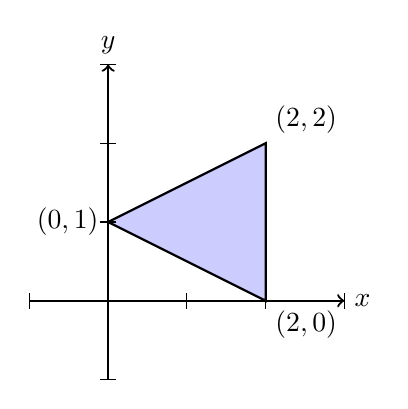
\begin{tikzpicture}[scale=1]
                      % Dibujar los ejes coordenados
                      \draw[->, thick] (-1, 0) -- (3, 0) node[right] {$x$}; % Eje x
                      \draw[->, thick] (0, -1) -- (0, 3) node[above] {$y$}; % Eje y

                      % Dibujar el triángulo
                      \draw[thick, fill=blue!20] (2, 0) -- (2, 2) -- (0, 1) -- cycle;

                      % Etiquetas para los vértices
                      \node at (2, 0) [below right] {$(2, 0)$};
                      \node at (2, 2) [above right] {$(2, 2)$};
                      \node at (0, 1) [left] {$(0, 1)$};

                      % Marcas en los ejes (sin números)
                      \foreach \x in {-1, 0, 1, 2, 3} {
                              \draw (\x, -0.1) -- (\x, 0.1); % Marcas en el eje x
                          }
                      \foreach \y in {-1, 0, 1, 2, 3} {
                              \draw (-0.1, \y) -- (0.1, \y); % Marcas en el eje y
                          }
                  \end{tikzpicture}
              \end{center}
              Intentemos
              calcular $$\int_D x^2y \,dx\,dy = \int_{\mathbb{R}^2} x^2y \cdot \chi_D
                  \,dx\,dy = \int_{x = -\infty}^{x = +\infty}(\int_{D_x}x^2\chi_Ddy)dx = $$
              Sabiendo que $D_x = \{y \in \mathbb{R} : (x,y) \in D\}$, si $0 \leq x \leq 2$
              entonces $D_x = \{y : -\frac{1}{2}x + 1 \leq y \leq \frac{1}{2}x+1\}$.\\ Por
              tanto, podemos plantear la integral como: $$= \int_{x = 0}^{x =2} \left(
                  \int_{y = -\frac{1}{2}x + 1}^{y = \frac{1}{2}x + 1} x^2y \,dy \right) dx =
                  \int_{0}^{2}x^2\left(\frac{1}{2}x + 1 + \frac{1}{2}x - 1\right)dx =
                  \int_{0}^{2}x^3dx = \frac{16}{4} = 4.$$\\ También podríamos haberlo planteado
              así, sabiendo que $D^y = \{x : (x,y) \in D\}$: $$\int_{y =0}^{y =
                      2}\left(\int_{D^y}x^2y \,dx\right)dy = \int_{y = 0}^{y = 1}\left(\int_{x =
                          2(1+y)}^{x =2}x^2y\,dx\right)dy + \int_{y = 1}^{y = 2}\left(\int_{x =
                          2(y-1)}^{x = 2}x^2y\,dx\right)dy.$$ Evaluamos:
              $$\int_{1}^{2}y\left(\int_{2(y-1)}^{2}x^2dx\right)dy =
                  \int_{1}^{2}y\left(\frac{8}{3}y^3 - 4y^2 + 4y\right)dy = \frac{1}{3}y^4 -
                  \frac{4}{3}y^3 + 2y^2 \Big|_{1}^{2} = 4.$$

              %2%
        \item Sea $D = \{(x,y) : 0 \leq x \leq y\}$ y $f(x,y) = xe^{-y^3}$. Calculemos:
              $$\int_{D}f(x,y)dxdy.$$ Dado que $f\geq 0$, podemos aplicar el Teorema de
              Tonelli: $$\int_{D}f(x,y)dxdy = \int_{\mathbb{R}^2}f\chi_D = \int_{x = 0}^{x =
                      +\infty}\left(\int_{y = x}^{y = +\infty}e^{-y^3}dy\right)dx.$$ No obstante, no
              conocemos el valor de la integral $\int_{y = x}^{y = +\infty}e^{-y^3}dy$, por
              lo que continuamos el cálculo en el otro sentido: $$\int_{y = 0}^{y =
                      +\infty}\left(e^{-y^3}\int_{x = 0}^{x = y}xdx\right)dy = \int_{y = 0}^{y =
                      +\infty}e^{-y^3}\left[\frac{x^2}{2}\right]^{x = y}_{x = 0}dy.$$ Evaluamos:
              $$\int_{y = 0}^{y = +\infty}e^{-y^3}\frac{y^2}{2}dy =
                  \left(-\frac{1}{2}\right)\frac{1}{3}\int_{y = 0}^{y = +\infty}e^{-y^3}(-3y^2)dy
                  = -\frac{1}{6}[e^{-y^3}]_{y = 0}^{y = +\infty}.$$

              %3%
        \item Sea $V$ el sólido limitado por $x = 0, \ y = 0, \ z = 0, \ 3x + 2y +z = 1$.
              Calculemos:
              \begin{enumerate}[label=(\alph*)]
                  \item $\text{Vol}(V)$
                  \item $\int_{V}z^2dxdydz$
              \end{enumerate}
              \vspace{-1.5cm}
              \begin{center}
                  \tdplotsetmaincoords{70}{120} % Ángulos para la perspectiva 3D
                  \begin{tikzpicture}[scale=2, tdplot_main_coords]
                      % Definir los ejes
                      \draw[->, thick] (0, 0, 0) -- (1.5, 0, 0) node[right] {$x$};
                      \draw[->, thick] (0, 0, 0) -- (0, 1.5, 0) node[above] {$y$};
                      \draw[->, thick] (0, 0, 0) -- (0, 0, 1.5) node[below left] {$z$};

                      % Definir los puntos de intersección del plano 3x + 2y + z = 1 con los ejes
                      \coordinate (A) at (1/3, 0, 0); % Intersección con el eje x
                      \coordinate (B) at (0, 1/2, 0); % Intersección con el eje y
                      \coordinate (C) at (0, 0, 1);   % Intersección con el eje z

                      % Dibujar el plano 3x + 2y + z = 1
                      \filldraw[fill=blue!20, opacity=0.7] (A) -- (B) -- (C) -- cycle;

                      % Dibujar las aristas del sólido
                      \draw[thick] (A) -- (B) -- (C) -- cycle;
                      \draw[thick] (0, 0, 0) -- (A);
                      \draw[thick] (0, 0, 0) -- (B);
                      \draw[thick] (0, 0, 0) -- (C);

                      % Etiquetas para los puntos de intersección
                      \node at (A) [above left] {$\left(\frac{1}{3}, 0, 0\right)$};
                      \node at (B) [above right] {$\left(0, \frac{1}{2}, 0\right)$};
                      \node at (C) [above left] {$\left(0, 0, 1\right)$};
                  \end{tikzpicture}

              \end{center}
              \begin{itemize}
                  \item[\textbf{(a)}]        Aplicamos el Lema de Cavalieri:
                        $$\text{Vol}(V) = \int_{\mathbb{R}^3} \chi_V(x,y,z)\,dx\,dy\,dz = \int_{z = 0}^{z = 1} \left(\int_{V_z}1dxdy\right)dz,$$
                        donde $V_z = \{(x,y) : (x,y,z) \in V\} = \{(x,y) : x \geq 0, y \geq 0, 3x + 2y \leq 1 - z\}$.

                        Definimos: $$\int_{z = 0}^{z = 1} \text{área}(V_z) dz,$$ donde el área de $V_z$
                        es: $$\text{área}(V_z) = \frac{1}{2} \cdot \frac{1-z}{3} \cdot \frac{1-z}{2}.$$
                        También se podría haber definido como: $$\int_{z = 0}^{z =1}\left(\int_{y =
                                0}^{y = \frac{1-z}{2}}\left(\int_{x = 0}^{x =
                                \frac{1-z-2y}{3}}1dx\right)dy\right)dz.$$ Otra forma alternativa de orden de
                        integración sería: $$\int_{y = 0}^{y = \frac{1}{2}}\left(\int_{z = 0}^{z =
                                    1}\left(\int_{x = 0}^{x = \frac{1-z-2y}{3}}1dx\right)dz\right)dy.$$
                  \item[\textbf{(b)}]  $$\int_{V}z^2dxdydz = \int_{z = 0}^{z = 1}z^2(\int_{V_z}1dxdy)dz = \int_{z = 0}^{z = 1}z^2\cdot\frac{(1-z)^2}{12}dz$$
              \end{itemize}
        \item Sea $V$ el sólido limitado por el paraboloide $z = x^2 +y^2$ y por el plano
              $z=1$.\\ Calculemos $vol(V)$.

              % remove a line
              \vspace{-1cm}

              \begin{center}
                  \tdplotsetmaincoords{75}{135}
                  \begin{tikzpicture}[tdplot_main_coords,scale=2.0]
                      \tikzmath{function f(\x) {return \x;};}
                      \pgfmathsetmacro{\zini}{0.5*sqrt(2.0)}
                      \pgfmathsetmacro{\step}{0.01}
                      \pgfmathsetmacro{\zsig}{\zini+\step}
                      \pgfmathsetmacro{\nextz}{\zini+0.5*\step}
                      \pgfmathsetmacro{\sig}{2.0*\step}
                      \pgfmathsetmacro{\tini}{0.5*pi}
                      \pgfmathsetmacro{\tfin}{1.85*pi}
                      \pgfmathsetmacro{\tend}{2.5*pi}
                      %%% Coordinate axis
                      \draw[thick,->] (0,0,0) -- (1.5,0,0) node [below left] {\footnotesize$x$};
                      \draw[dashed] (0,0,0) -- (-1.5,0,0);
                      \draw[thick,->] (0,0,0) -- (0,1.5,0) node [right] {\footnotesize$y$};
                      \draw[dashed] (0,0,0) -- (0,-1.5,0);
                      \draw[thick] (0,0,0) -- (0,0,1.0); % Z axis (part under the plane z = 1)
                      % The region of integration
                      \draw[gray,thick,fill=yellow!20,opacity=0.75] plot[domain=0:6.2832,smooth,variable=\t] ({1.0*cos(\t r)},{1.0*sin(\t r)},{0.0});
                      %	
                      \draw[gray,dash dot dot] (-1,0,0) -- (-1,0,1);
                      \draw[gray,dash dot dot] (0,-1,0) -- (0,-1,1);
                      % The plane: x + y = 1
                      \coordinate (A) at (1,1,1);
                      \coordinate (B) at (-1,1,1);
                      \coordinate (C) at (-1,-1,1);
                      \coordinate (D) at (1,-1,1);
                      % Curves bounding the solid.
                      \draw[blue,thick,opacity=0.5] plot[domain=-1:1,smooth,variable=\t] ({\t},0,{\t*\t});
                      \draw[blue,thick,opacity=0.5] plot[domain=-1:1,smooth,variable=\t] (0,{\t},{\t*\t});
                      \draw[blue,thick,opacity=0.5] plot[domain=0:6.2832,smooth,variable=\t] ({1.0*cos(\t r)},{1.0*sin(\t r)},{1.0});
                      % The paraboloid (level curves z = constant)
                      \foreach \altura in {\step,\sig,...,1.0}{
                              \pgfmathparse{sqrt(\altura)}
                              \pgfmathsetmacro{\radio}{\pgfmathresult}
                              \draw[blue!20,thick,opacity=0.5] plot[domain=0:6.2832,smooth,variable=\t] ({\radio*cos(\t r)},{\radio*sin(\t r)},{\altura});
                          }
                      % The plane
                      \draw[white] (C) -- (B) node[red,above,sloped,midway]{$z = 1$};
                      \fill[pattern color=pink,pattern=north east lines] (A) -- (B) -- (C) -- (D) -- (A);
                      \draw[thick,red] (A) -- (B) -- (C) -- (D) -- (A);
                      %
                      \draw[gray,dash dot dot] (1,0,0) -- (1,0,1);
                      \draw[gray,dash dot dot] (0,1,0) -- (0,1,1);
                      %
                      \node[blue,left] at (0.5,-0.75,0.5) {$z = x^2 + y^2$};
                      \draw[thick,->] (0,0,1.0) -- (0,0,1.5) node [above] {\footnotesize$z$};
                  \end{tikzpicture}
              \end{center}

              Donde $$V = \{(x,y,z) \in \mathbb{R}^3 : x^2 + y^2 \leq z \leq 1\} \implies
                  \\$$ $$vol(v) = \int_{z = 0}^{z = 1}area(V_z)dz = \int_{0}^{1}\pi z dz =
                  \frac{\pi}{2}$$. \\
    \end{enumerate}
}

\begin{observación}
La diferencia entre el Teorema de Tonelli y el de Fubini, es que el primero pide que las funciones sean no-negativas estrictamente y el segundo pide que las funciones sean integrables absolutamente.
\end{observación}

\begin{definición} [Conjunto Verticalmente Proyectable\label{Conjunto Verticalmente Proyectable}]
Un conjunto $E \subset \mathbb{R}^2$ es verticalmente proyectable si es de la forma:
$$E_1 = \{(x,y) : a \leq x \leq b, f(x) \leq y \leq g(x)\}$$ donde $f,g : [a,b] \to \mathbb{R}$ son funciones continuas con $f(x) \leq g(x)$.
Análogamente se define un conjunto $E \subset \mathbb{R}^2$ es horizontalmente proyectable si es de la forma:
$$E_2 = \{ (x,y) : c \leq y \leq d, \varphi(y) \leq x \leq \psi(y)\}$$
donde $\varphi, \psi : [c,d] \to \mathbb{R}$ son funciones continuas con $\varphi(y) \leq \psi(y)$.
En este caso si $f: E \to \mathbb{R}$ que es integrable en $E$:
$$\int_{E_1}h(x,y)dxdy = \int_{x = a}^{x = b}\left(\int_{f(x)}^{g(x)}h(x,y)dy\right)dx$$
$$\int_{E_2}h(x,y)dxdy = \int_{y = c}^{y = d}\left(\int_{\varphi(y)}^{\psi(y)}h(x,y)dx\right)dy$$

\begin{center}
    \begin{minipage}{0.45\textwidth}
        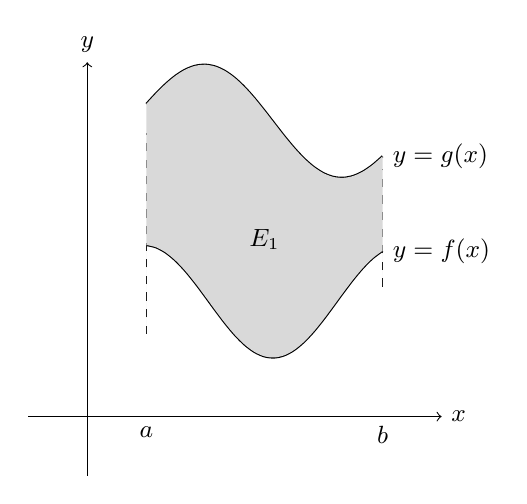
\begin{tikzpicture}[scale=1.5]
            % Ejes
            \draw[->] (-0.5,0) -- (3,0) node[right] {\small $x$};
            \draw[->] (0,-0.5) -- (0,3) node[above] {\small $y$};

            % Curvas más variadas
            \draw[thick, domain=0.5:2.5, smooth, variable=\x] plot ({\x}, {1 + 0.4*sin(3*\x r) + 0.1*cos(2*\x r)}) node[right] {\small $y = f(x)$}; % Ajuste aquí
            \draw[thick, domain=0.5:2.5, smooth, variable=\x] plot ({\x}, {2.5 - 0.3*cos(3*\x r) + 0.2*sin(2*\x r)}) node[right] {\small $y = g(x)$};

            % Líneas verticales en x=a y x=b
            \draw[dashed] (0.5,0.7) -- (0.5,2.4);
            \draw[dashed] (2.5,1.1) -- (2.5,2.1);

            % Etiquetas a y b
            \node[below] at (0.5,0) {\small $a$};
            \node[below] at (2.5,0) {\small $b$};

            % Región sombreada
            \begin{scope}
                \clip (0.5,0.7) -- plot[domain=0.5:2.5, smooth] (\x, {2.5 - 0.3*cos(3*\x r) + 0.2*sin(2*\x r)}) -- (2.5,1.1) -- plot[domain=2.5:0.5, smooth] (\x, {1 + 0.4*sin(3*\x r) + 0.1*cos(2*\x r)}) -- cycle; % Ajuste aquí
                \fill[gray!30] (0,0) rectangle (3,3);
            \end{scope}

            % Etiqueta de la región
            \node at (1.5,1.5) {\small $E_1$};

        \end{tikzpicture}
    \end{minipage}
    \hspace{0.05\textwidth} % Espacio entre las dos figuras
    \begin{minipage}{0.45\textwidth}

        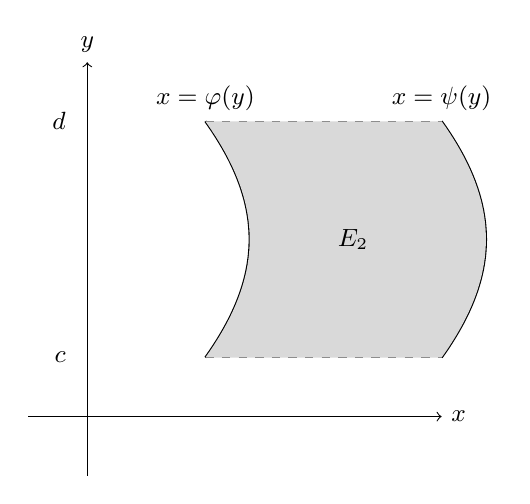
\begin{tikzpicture}[scale=1.5]
            % Ejes de coordenadas con una separación más pequeña
            \draw[->] (-0.5,0) -- (3,0) node[right] {\small $x$};
            \draw[->] (0,-0.5) -- (0,3) node[above] {\small $y$};

            \node[left] at (-0.1,0.5) {\small $c$};  % Etiqueta en y = 0.5
            \node[left] at (-0.1,2.5) {\small $d$};  % Etiqueta en y = 2.5

            % Mover la figura ligeramente a la derecha
            \begin{scope}[shift={(1,0)}]  % Ahora solo 1 unidad a la derecha
                \draw[thick] (0,0.5) .. controls (0.5,1.2) and (0.5,1.8) .. (0,2.5)
                node[above] {\small $x = \varphi(y)$};

                \draw[thick] (2,0.5) .. controls (2.5,1.2) and (2.5,1.8) .. (2,2.5)
                node[above] {\small $x = \psi(y)$};

                % Líneas horizontales
                \draw[dashed] (0,0.5) -- (2,0.5);
                \draw[dashed] (0,2.5) -- (2,2.5);

                % Región sombreada
                \fill[gray!30] (0,0.5) .. controls (0.5,1.2) and (0.5,1.8) .. (0,2.5) --
                (2,2.5) .. controls (2.5,1.8) and (2.5,1.2) .. (2,0.5) -- cycle;

                \node at (1.25,1.5) {\small $E_2$};
            \end{scope}
        \end{tikzpicture}

    \end{minipage}
\end{center}
\end{definición}

\begin{observación}
La diferencia entre ambas definciones es que en la primera se fija $x$ y se mueve $y$ y en la segunda se fija $y$ y se mueve $x$. Lo que tiene como consecuencia que en la primera se integra $dx-dy$ y en la segunda $dy-dx$.
\end{observación}

\begin{teorema}
    Sea $T: \mathbb{R}^n \to \mathbb{R}^n$ aplicación lineal. Sea $A \subset \mathbb{R}^n$ medible $\implies T(A)$ es medible y además:
    \[m(T(A)) = |\det(T)|m(A)\]
\end{teorema}
\begin{definición} [Difeomorfismo\label{difeomorfismo}]
Sean $U, V \subset \mathbb{R}^n$ abiertos se dice que $\varphi: U \to V$ es un difeomorfismo de $U$ a $V$ si:
\vspace{-0.5em}
\begin{enumerate}
    \item $\varphi$ es biyectiva
    \item $\varphi$ es de clase $C^1$ en $U$
    \item $\varphi^{-1}$ es de clase $C^1$ en $V$
\end{enumerate}
\end{definición}
\begin{observación}
Sea $\varphi: U \to \mathbb{R}$ de clase $C^1$ donde $U \subset \mathbb{R}^n$ es abierto, y supongamos que $det(D\varphi(u)) \neq 0 \quad \forall u \in U \implies V = \varphi(U)$ es abierto. Si $\varphi$ es inyectiva, tenemos que $\varphi: U \to \varphi(U) = V$ es un difeomorfismo.
\end{observación}

\begin{teorema}
    Sean $U, V \subset \mathbb{R}^n$ abierto y $\varphi: U \to V$ difeomorfismo-$C^{1}$. Si $A \subset U$ es medible, entonces $\varphi(A)$ es medible y $m(\varphi(A)) = \int_{A}|\det(D\varphi(u))|du$.
\end{teorema}

\begin{teorema}[Teorema del Cambio de Variable\label{TCV}]
    Sean $U,V \subset \mathbb{R}^n$ abiertos y $\varphi: U \to V$ difeomorfismo-$C^1$. Sea $f: V \to \mathbb{R}$ medible. Entonces:
    \begin{enumerate}
        \item Si $f$ es no negativa $\implies (f \circ \varphi) |\det(D\varphi)|$ es medible
              y no-negativa.
        \item Si $f$ es integrable $\implies (f \circ \varphi)|\det(D\varphi)|$ es integrable \end{enumerate}
    En ambos casos se cumple que:
    $$\int_{V = \varphi(U)} f(x)dx = \int_U (f \circ \phi(u))|\det(D\varphi)|du$$
\end{teorema}
\begin{observación}
Si $A \subset U$ es medible $\implies \varphi(A)$ es medible y
$$\int_{\varphi(A)}f(x)dx = \int_{A}(f \circ \varphi(u))|\det(D\varphi)|du$$
\end{observación}

\ejemplo{
    Sea $\int_{E} e^{\frac{x-y}{x+y}}dxdy$ donde $E = $ tríangulo de vértices $(0,0), (2,0)$ y $(0,2)$.\\
    Si tomamos el cambio de variable: \\ $$\varphi^{-1} \begin{cases} u = x-y \\ v = x+y \end{cases} \implies \varphi \begin{cases} x = \frac{u+v}{2} \\ y = \frac{v - u}{2} \end{cases} \implies f(x,y) = f(u,v) = e^{\frac{u}{v}}$$\\
    Si tomamos la representación gráfica del cambio de variable obtenemos que:
    \begin{center}
        \begin{minipage}{0.45\textwidth}
            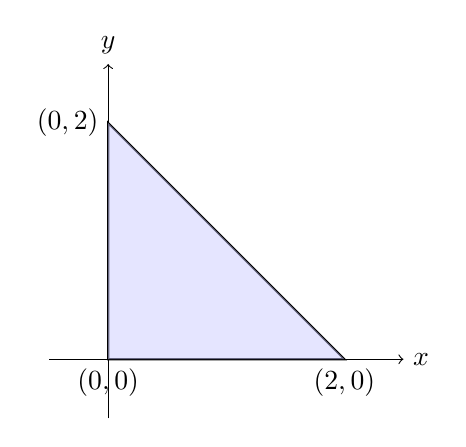
\begin{tikzpicture}[scale=1.5]
                % Ejes coordenados
                \draw[->] (-0.5,0) -- (2.5,0) node[right] {$x$}; % Dibuja el eje x con una flecha en el extremo derecho
                \draw[->] (0,-0.5) -- (0,2.5) node[above] {$y$}; % Dibuja el eje y con una flecha en el extremo superior

                % Triángulo original en xy
                \draw[thick] (0,0) -- (2,0) -- (0,2) -- cycle; % Dibuja el triángulo con vértices en (0,0), (2,0) y (0,2)

                % Etiquetas de los vértices
                \node[below] at (0,0) {$(0,0)$}; % Etiqueta el vértice (0,0)
                \node[below] at (2,0) {$(2,0)$}; % Etiqueta el vértice (2,0)
                \node[left] at (0,2) {$(0,2)$}; % Etiqueta el vértice (0,2)

                % Área sombreada
                \fill[blue!20,opacity=0.5] (0,0) -- (2,0) -- (0,2) -- cycle; % Rellena el triángulo con un color azul claro y opacidad del 50%
            \end{tikzpicture}
        \end{minipage}
        \hspace{0.0000001\textwidth} % Ajusta este valor para cambiar la separación entre las dos minipages
        \begin{minipage}{0.45\textwidth}
            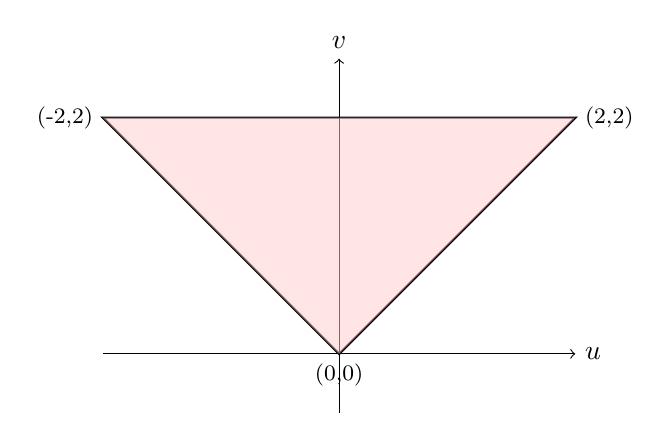
\begin{tikzpicture}[scale=1.5]
                % Ejes coordenados
                \draw[->] (-2,0) -- (2,0) node[right] {$u$};
                \draw[->] (0,-0.5) -- (0,2.5) node[above] {$v$};

                % Triángulo
                \draw[thick] (-2,2) -- (2,2) -- (0,0) -- cycle;

                % Etiquetas de los vértices
                \node[left] at (-2,2) {\footnotesize (-2,2)};
                \node[right] at (2,2) {\footnotesize (2,2)};
                \node[below] at (0,0) {\footnotesize (0,0)};

                \fill[red!20,opacity=0.5] (0,0) -- (2,2) -- (-2,2) -- cycle; % Rellena el triángulo transformado con un color rojo claro y opacidad del 50%
            \end{tikzpicture}
        \end{minipage}
    \end{center}

    Si tomamos $y = 0 \implies \varphi^{-1} \begin{cases} u = x \\ v = x \end{cases}$ y también tomamos $x = 0 \implies \begin{cases} u = -y \\ v = y \end{cases}$\\
    en tenemos que $|det(D\varphi)| = \begin{bmatrix} \frac{1}{2} & \frac{1}{2} \\ -\frac{1}{2} & \frac{1}{2} \end{bmatrix} = \frac{1}{2}$\\
    $$\int_{E}f(x,y)dxdy = \int_D e^{\frac{u}{v}} |det(D\varphi)du dv = \int_D \frac{1}{2} e^{\frac{u}{v}}du dv = \frac{1}{2} \int_{v = 0}^{v = 2}\left(\int_{u = -v}^{u = v}e^{\frac{u}{v}}du\right)dv$$
    $$  = \frac{1}{2} \int_{v = 0}^{v = 2}\left[v e^{\frac{u}{v}}\right] _{u = -v}^{u = v} dv = \frac{1}{2} \int_{v = 0}^{v =2}v(e-\frac{1}{e})dv = \frac{1}{2}(e-e^{-1}) \left[\frac{v^2}{2}\right]_{v = 0}^{v=2} = e - e^{-1}$$
}

